\section{پیاده‌سازی کنترل‌کننده \lr{LQIDG} روی استند سه درجه آزادی}\label{3DOF_lqidg_section}
در بخش‌های
\ref{lin_MIMO}
و
\ref{lin_SISO}،
فرم خطی فضای حالت چهارپره و فرم خطی فضای حالت کانال‌های چهارپره محاسبه شده‌است. در بخش‌های
\ref{lqidg_siso}
و
\ref{lqidg_mimo}
به‌ترتیب پیاده‌سازی به‌صورت سه کانال تک ورودی و چند ورودی انجام شده‌است.

%\subsection{پیاده‌سازی کنترل‌کننده \lr{LQIDG} بر رویه استند به‌صورت سه کانال تک ورودی}
\subsection{پیاده‌سازی کنترل‌کننده به‌صورت سه کانال تک ورودی}\label{lqidg_siso}
در بخش
\ref{roll_pitch_yaw_lqidg_section_ll}
شبیه‌سازی سه درجه آزادی استند چهارپره در حضور کنترل‌کننده \lr{LQIDG} انجام شد. در این بخش به پیاده‌سازی کنترل‌کننده \lr{LQIDG} روی استند سه درجه آزادی پرداخته شده‌است.
در پیاده‌سازی از ضرایب وزنی بهینه به دست آمده در قسمت شبیه‌سازی استفاده شده‌است.


\begin{figure}[H]
	\centering
	\subfigure[تغییرات زاویه رول]{
		\centering
		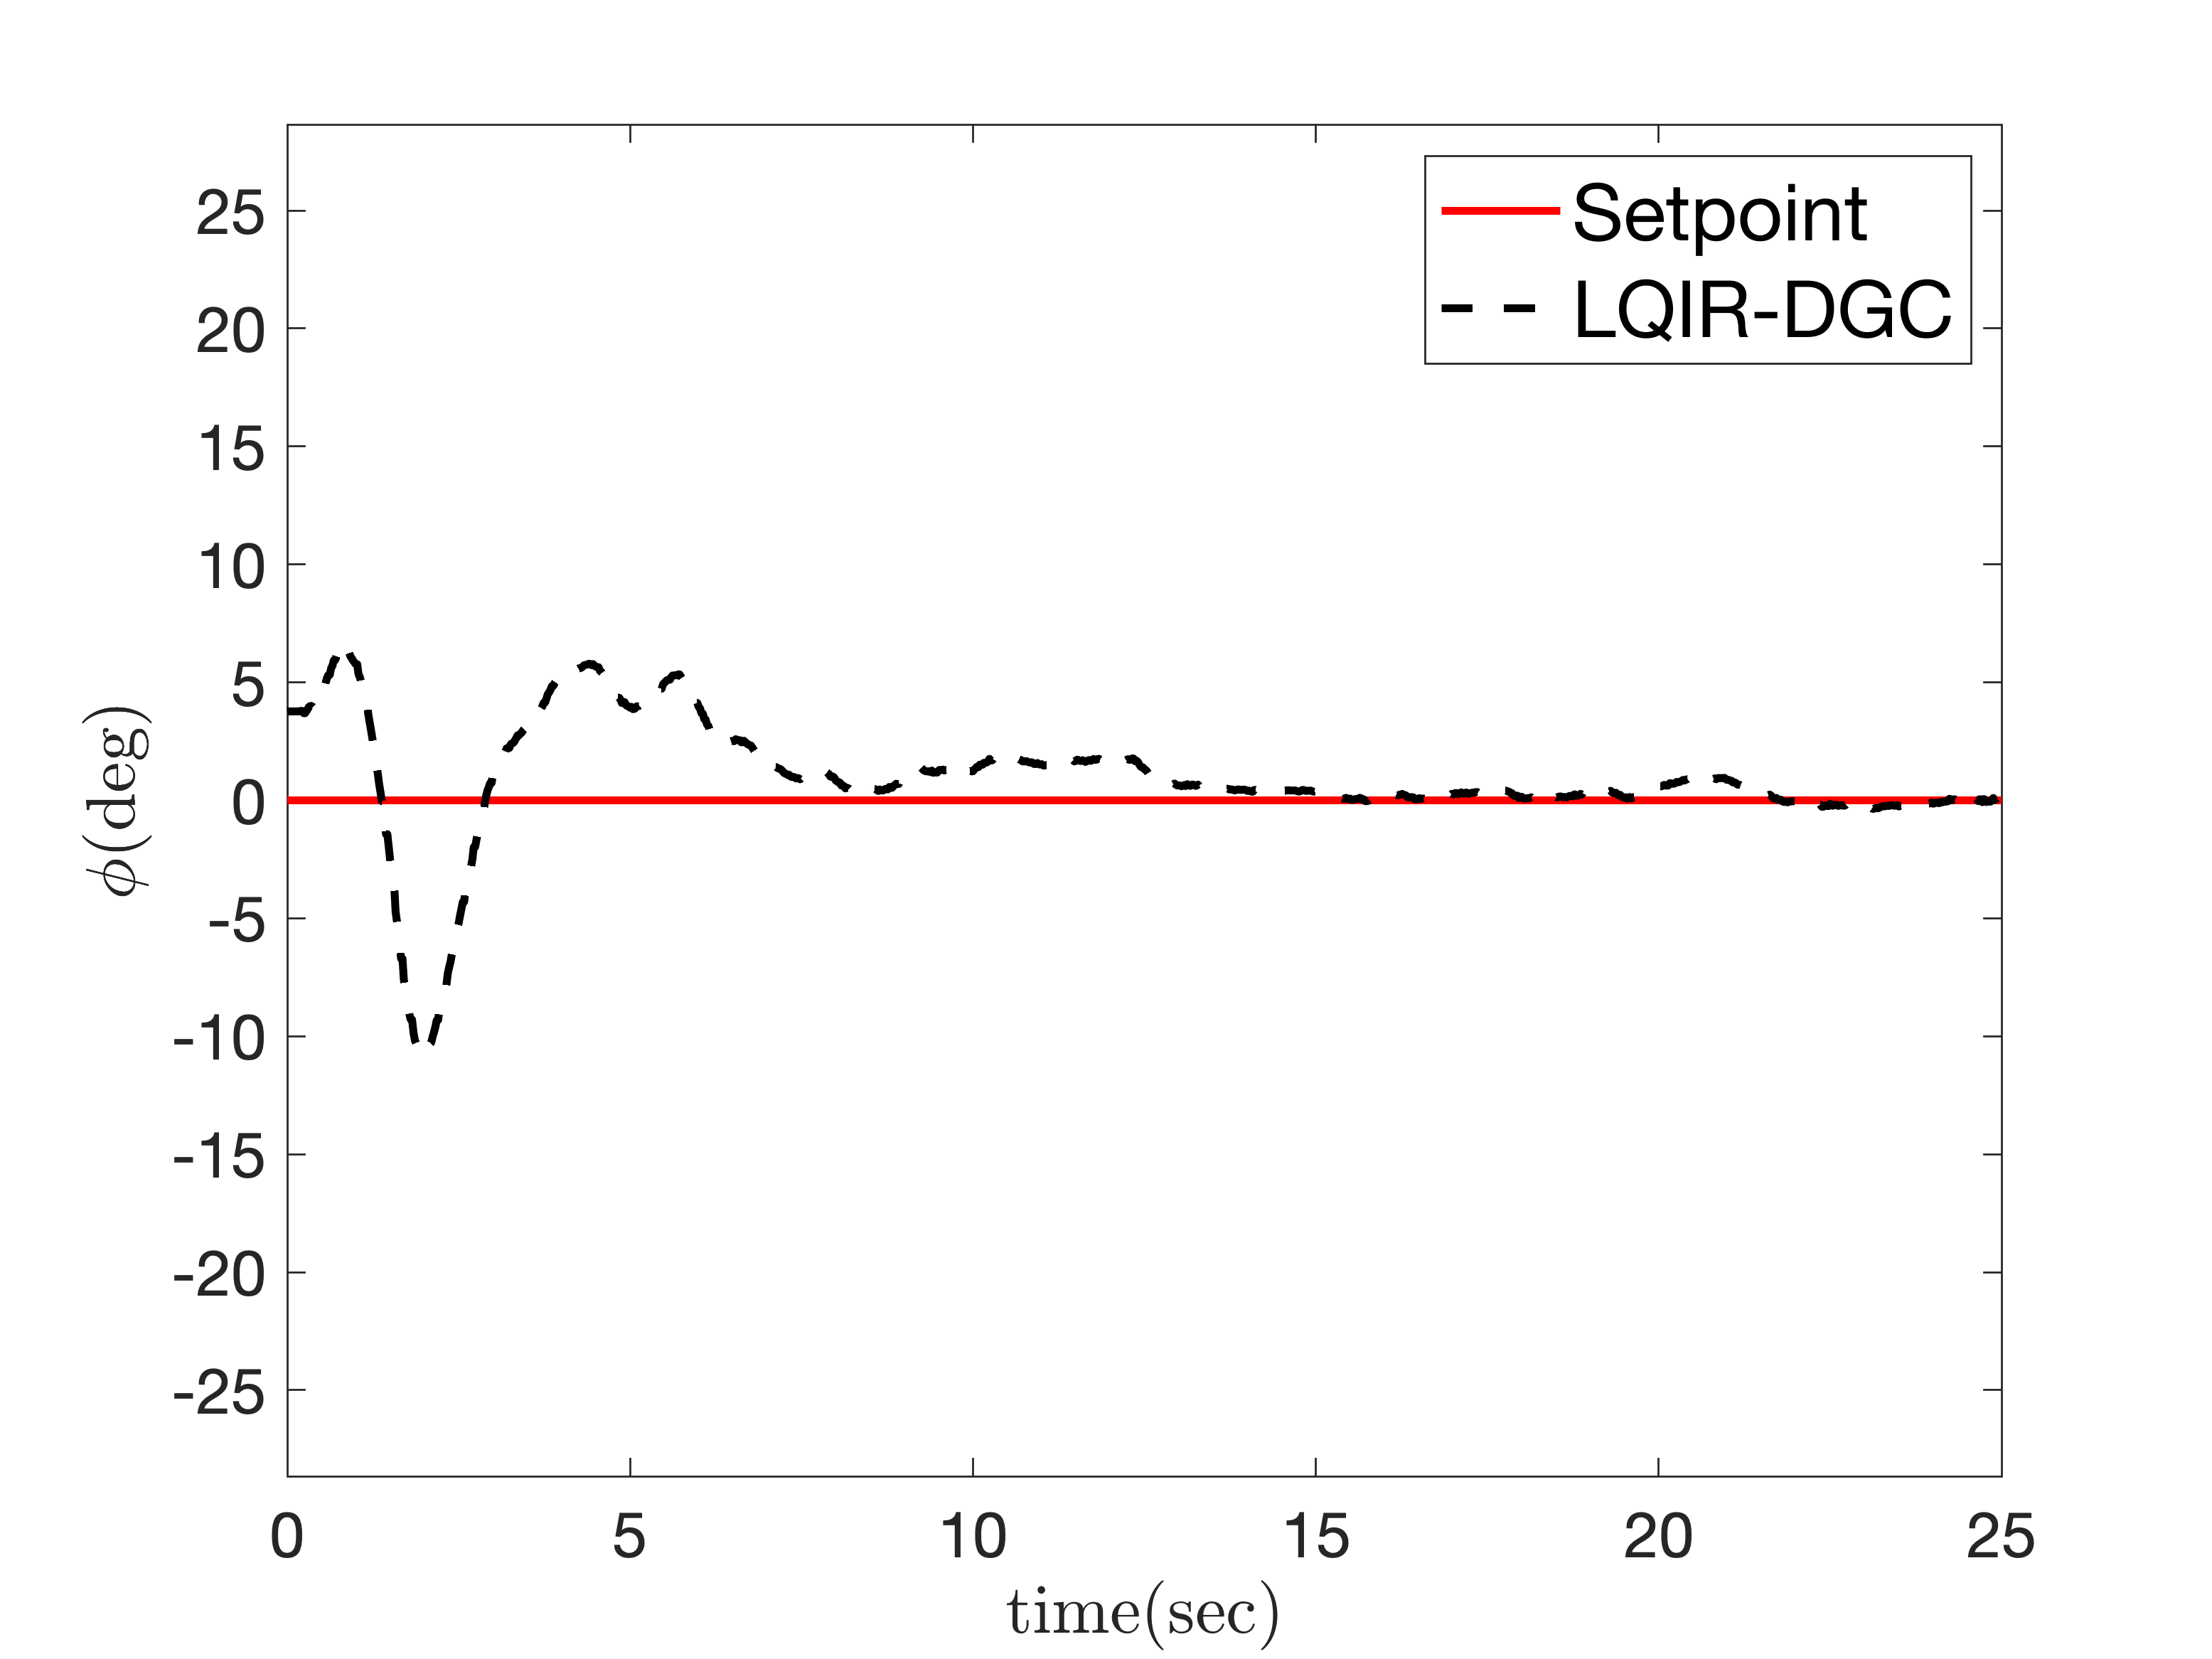
\includegraphics[width=.48\linewidth]{../Figures/Calibration/LQIDG/3DOF/lqidg_roll.png}
	}
	\subfigure[تغییرات زاویه پیچ]{
		\centering
		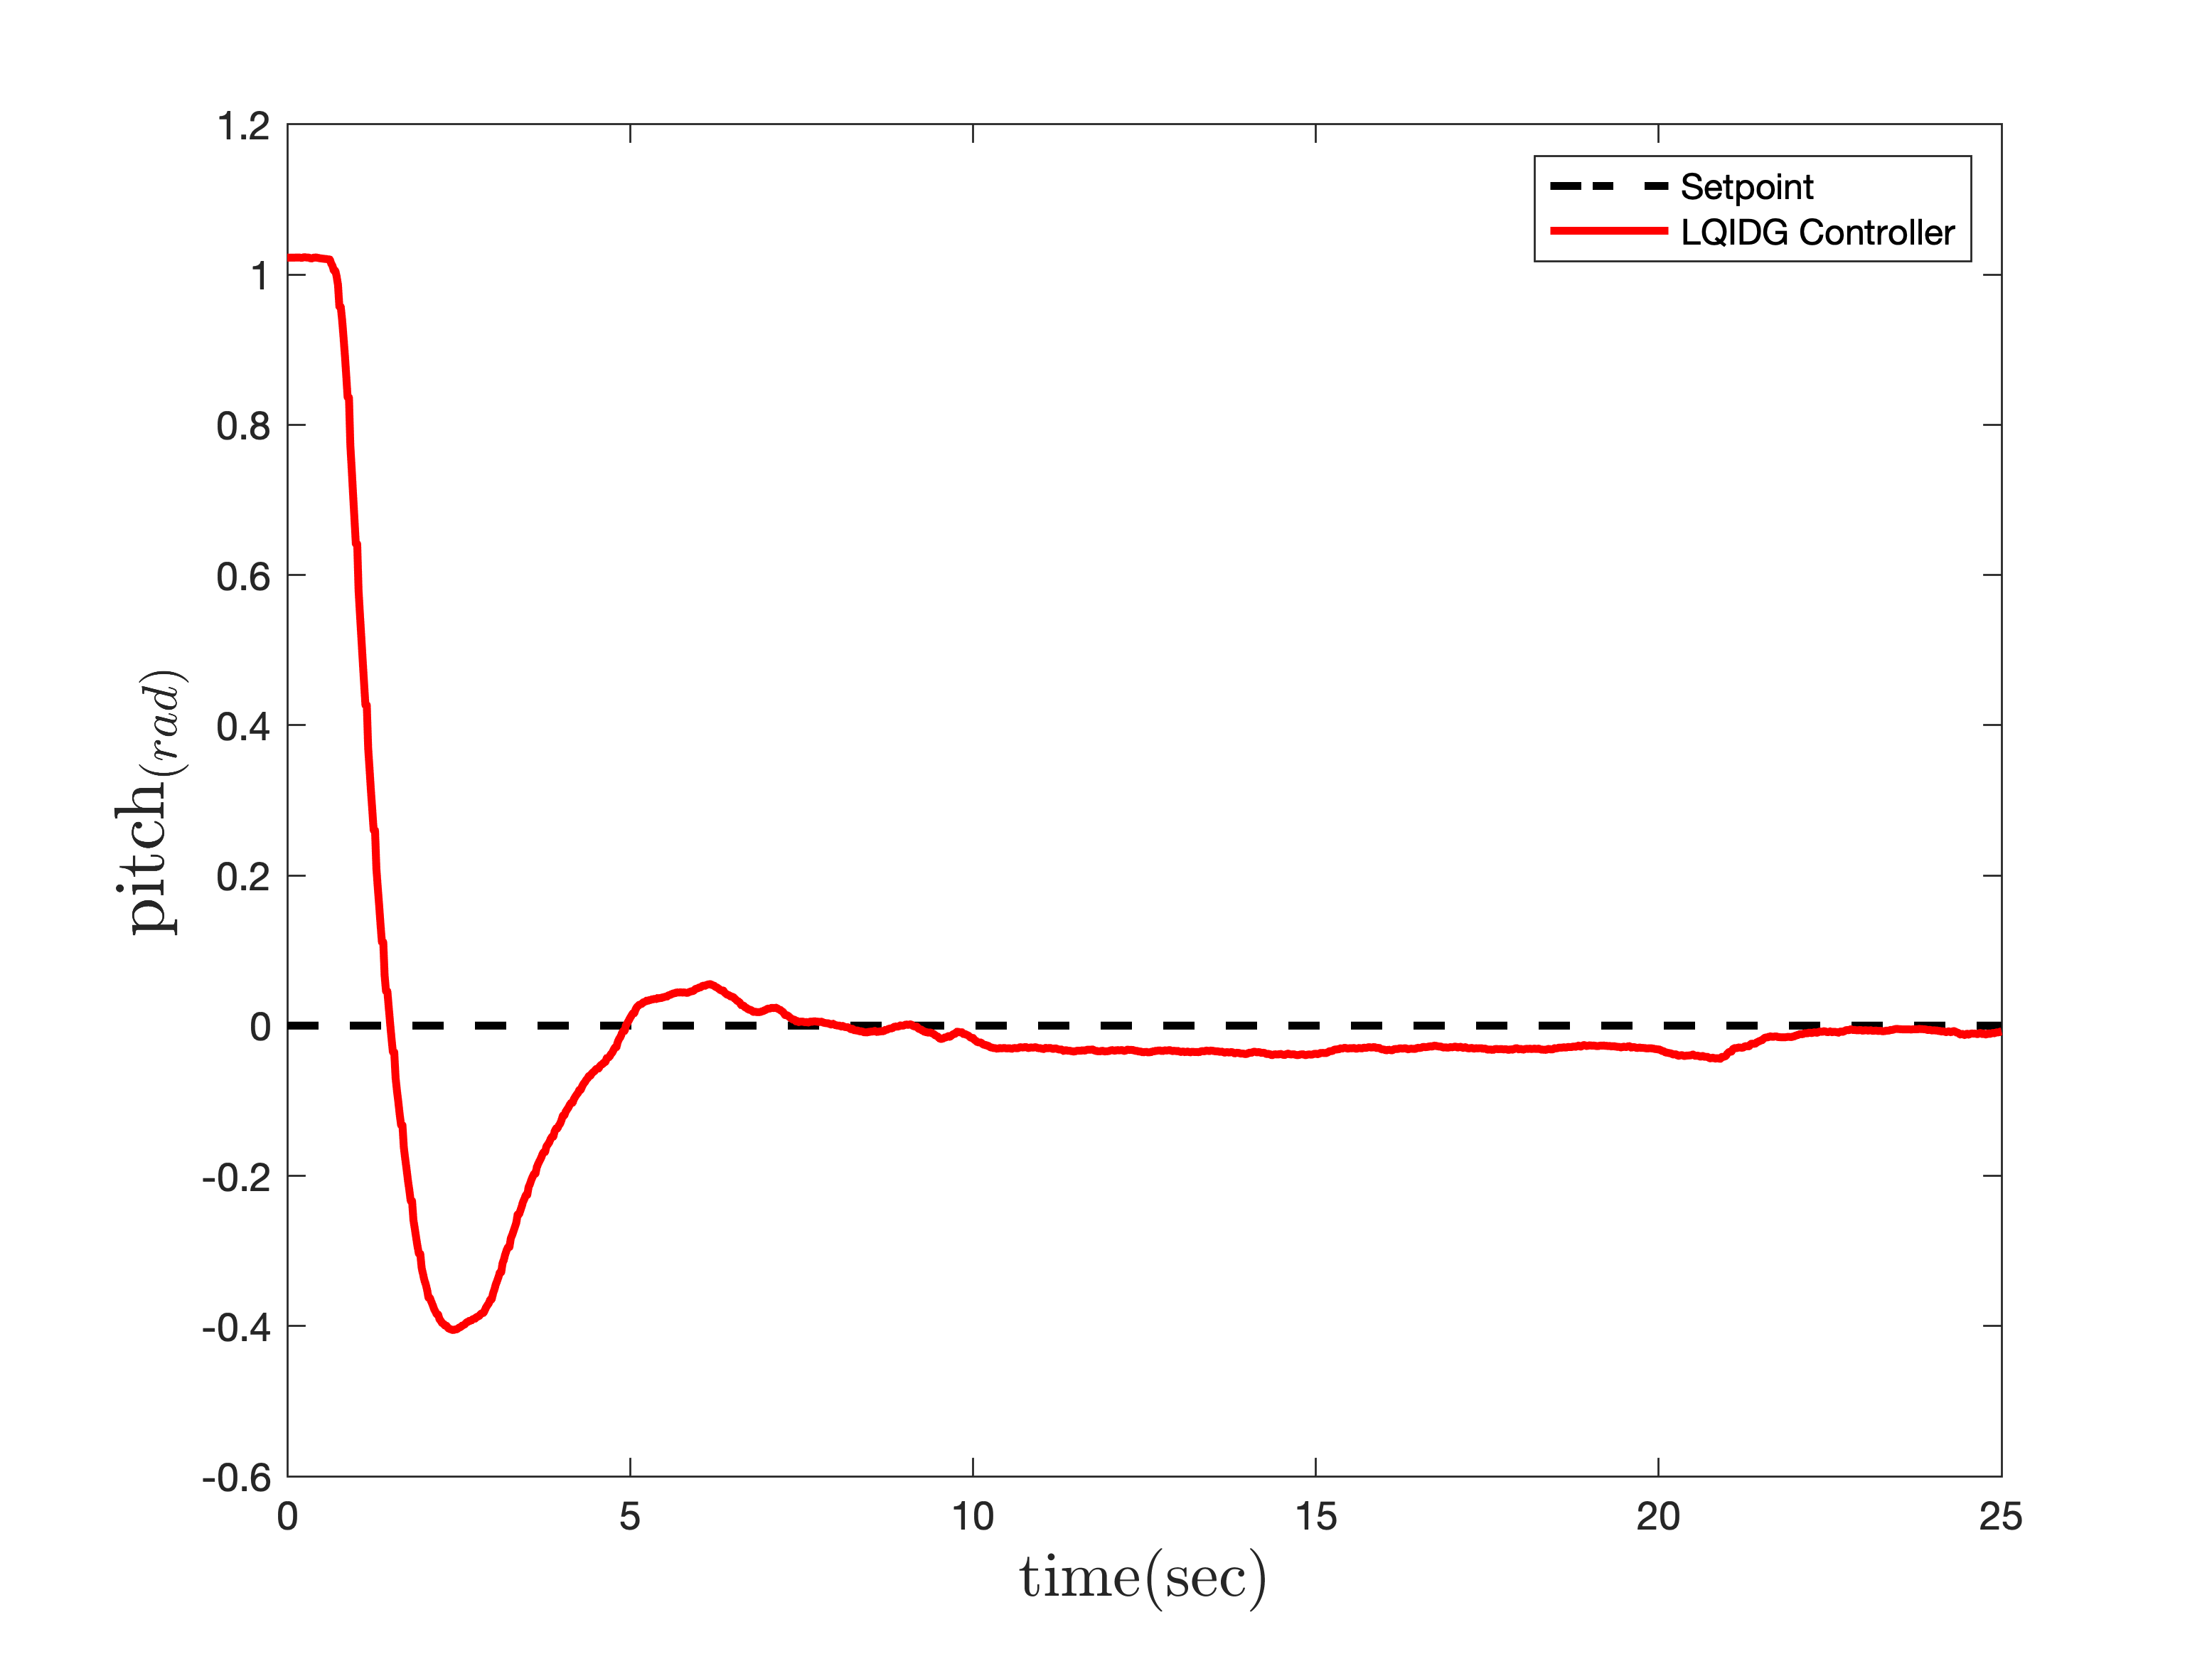
\includegraphics[width=.48\linewidth]{../Figures/Calibration/LQIDG/3DOF/lqidg_pitch.png}
	}
	\subfigure[تغییرات زاویه یاو]{
	\centering
	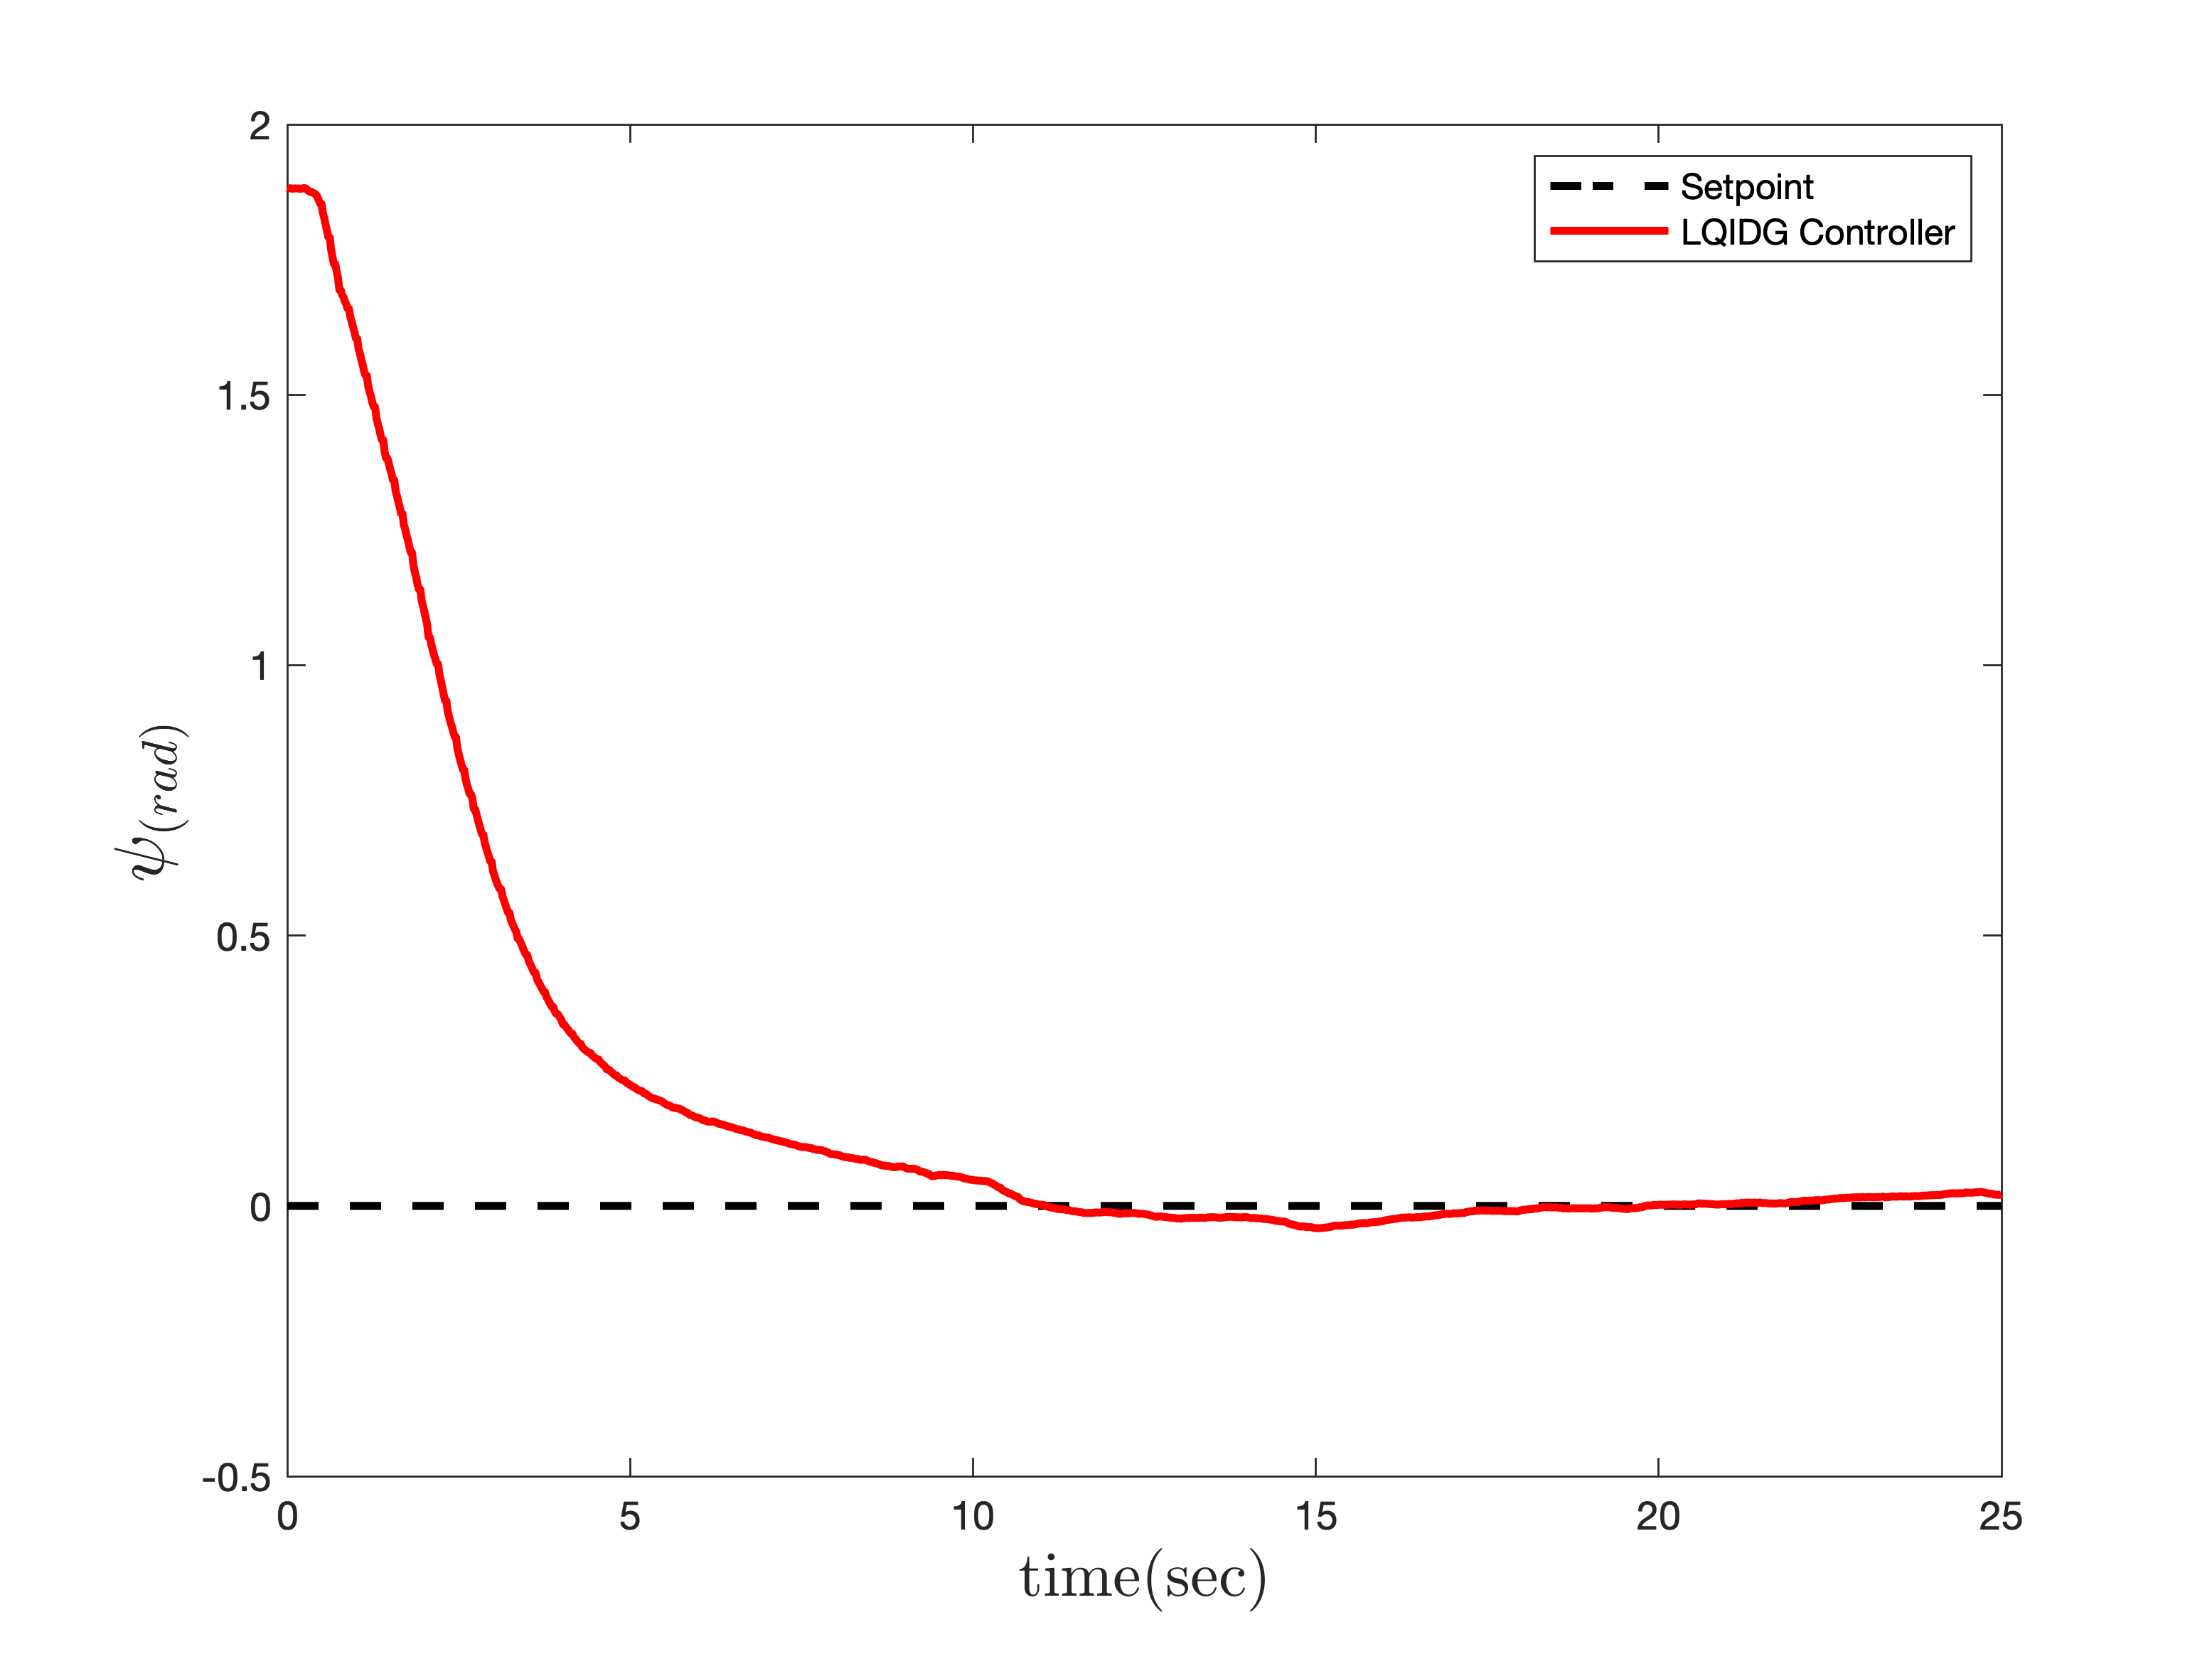
\includegraphics[width=.48\linewidth]{../Figures/Calibration/LQIDG/3DOF/lqidg_yaw.png}
}
	\caption{‫‪عملکرد کنترل‌کننده \lr{LQIDG} در کنترل وضعیت (تعقیب ورودی صفر)}
\end{figure}



\begin{figure}[H]
	\centering
	\subfigure[موتور شماره یک]{
		\centering
		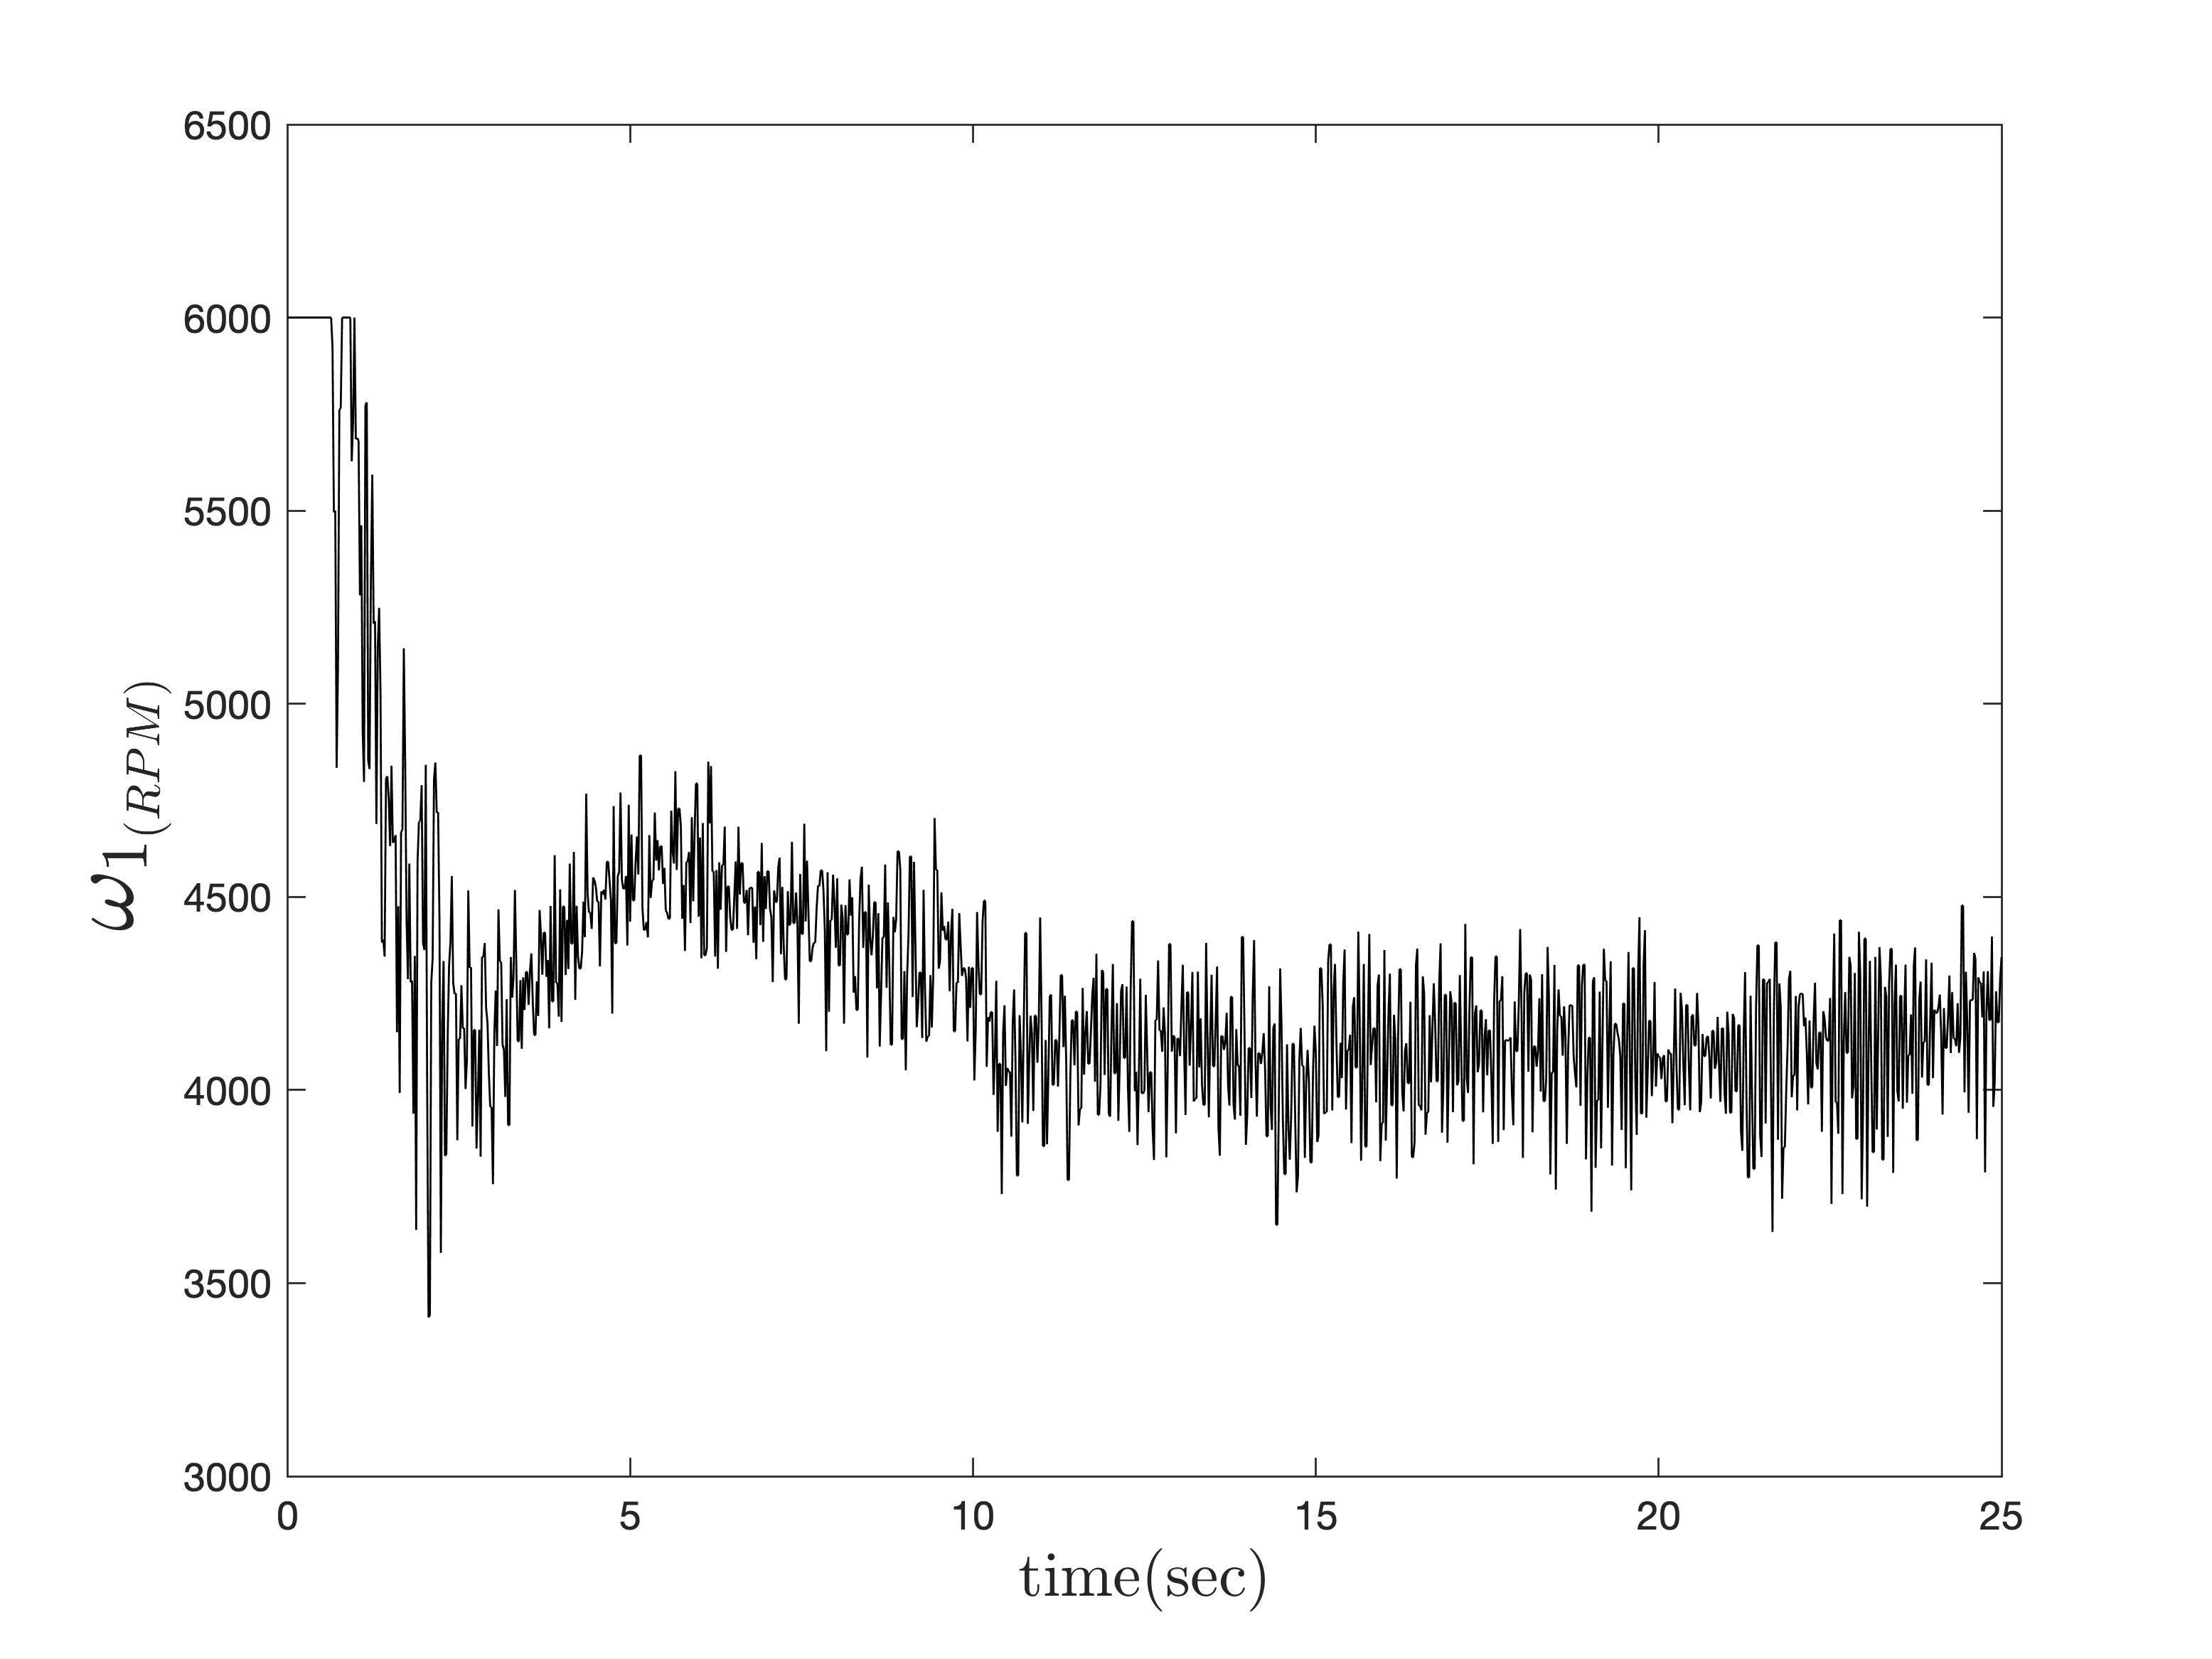
\includegraphics[width=.45\linewidth]{../Figures/Calibration/LQIDG/3DOF/lqidg_Omega_1.png}
	}
	\subfigure[موتور شماره دو]{
		\centering
		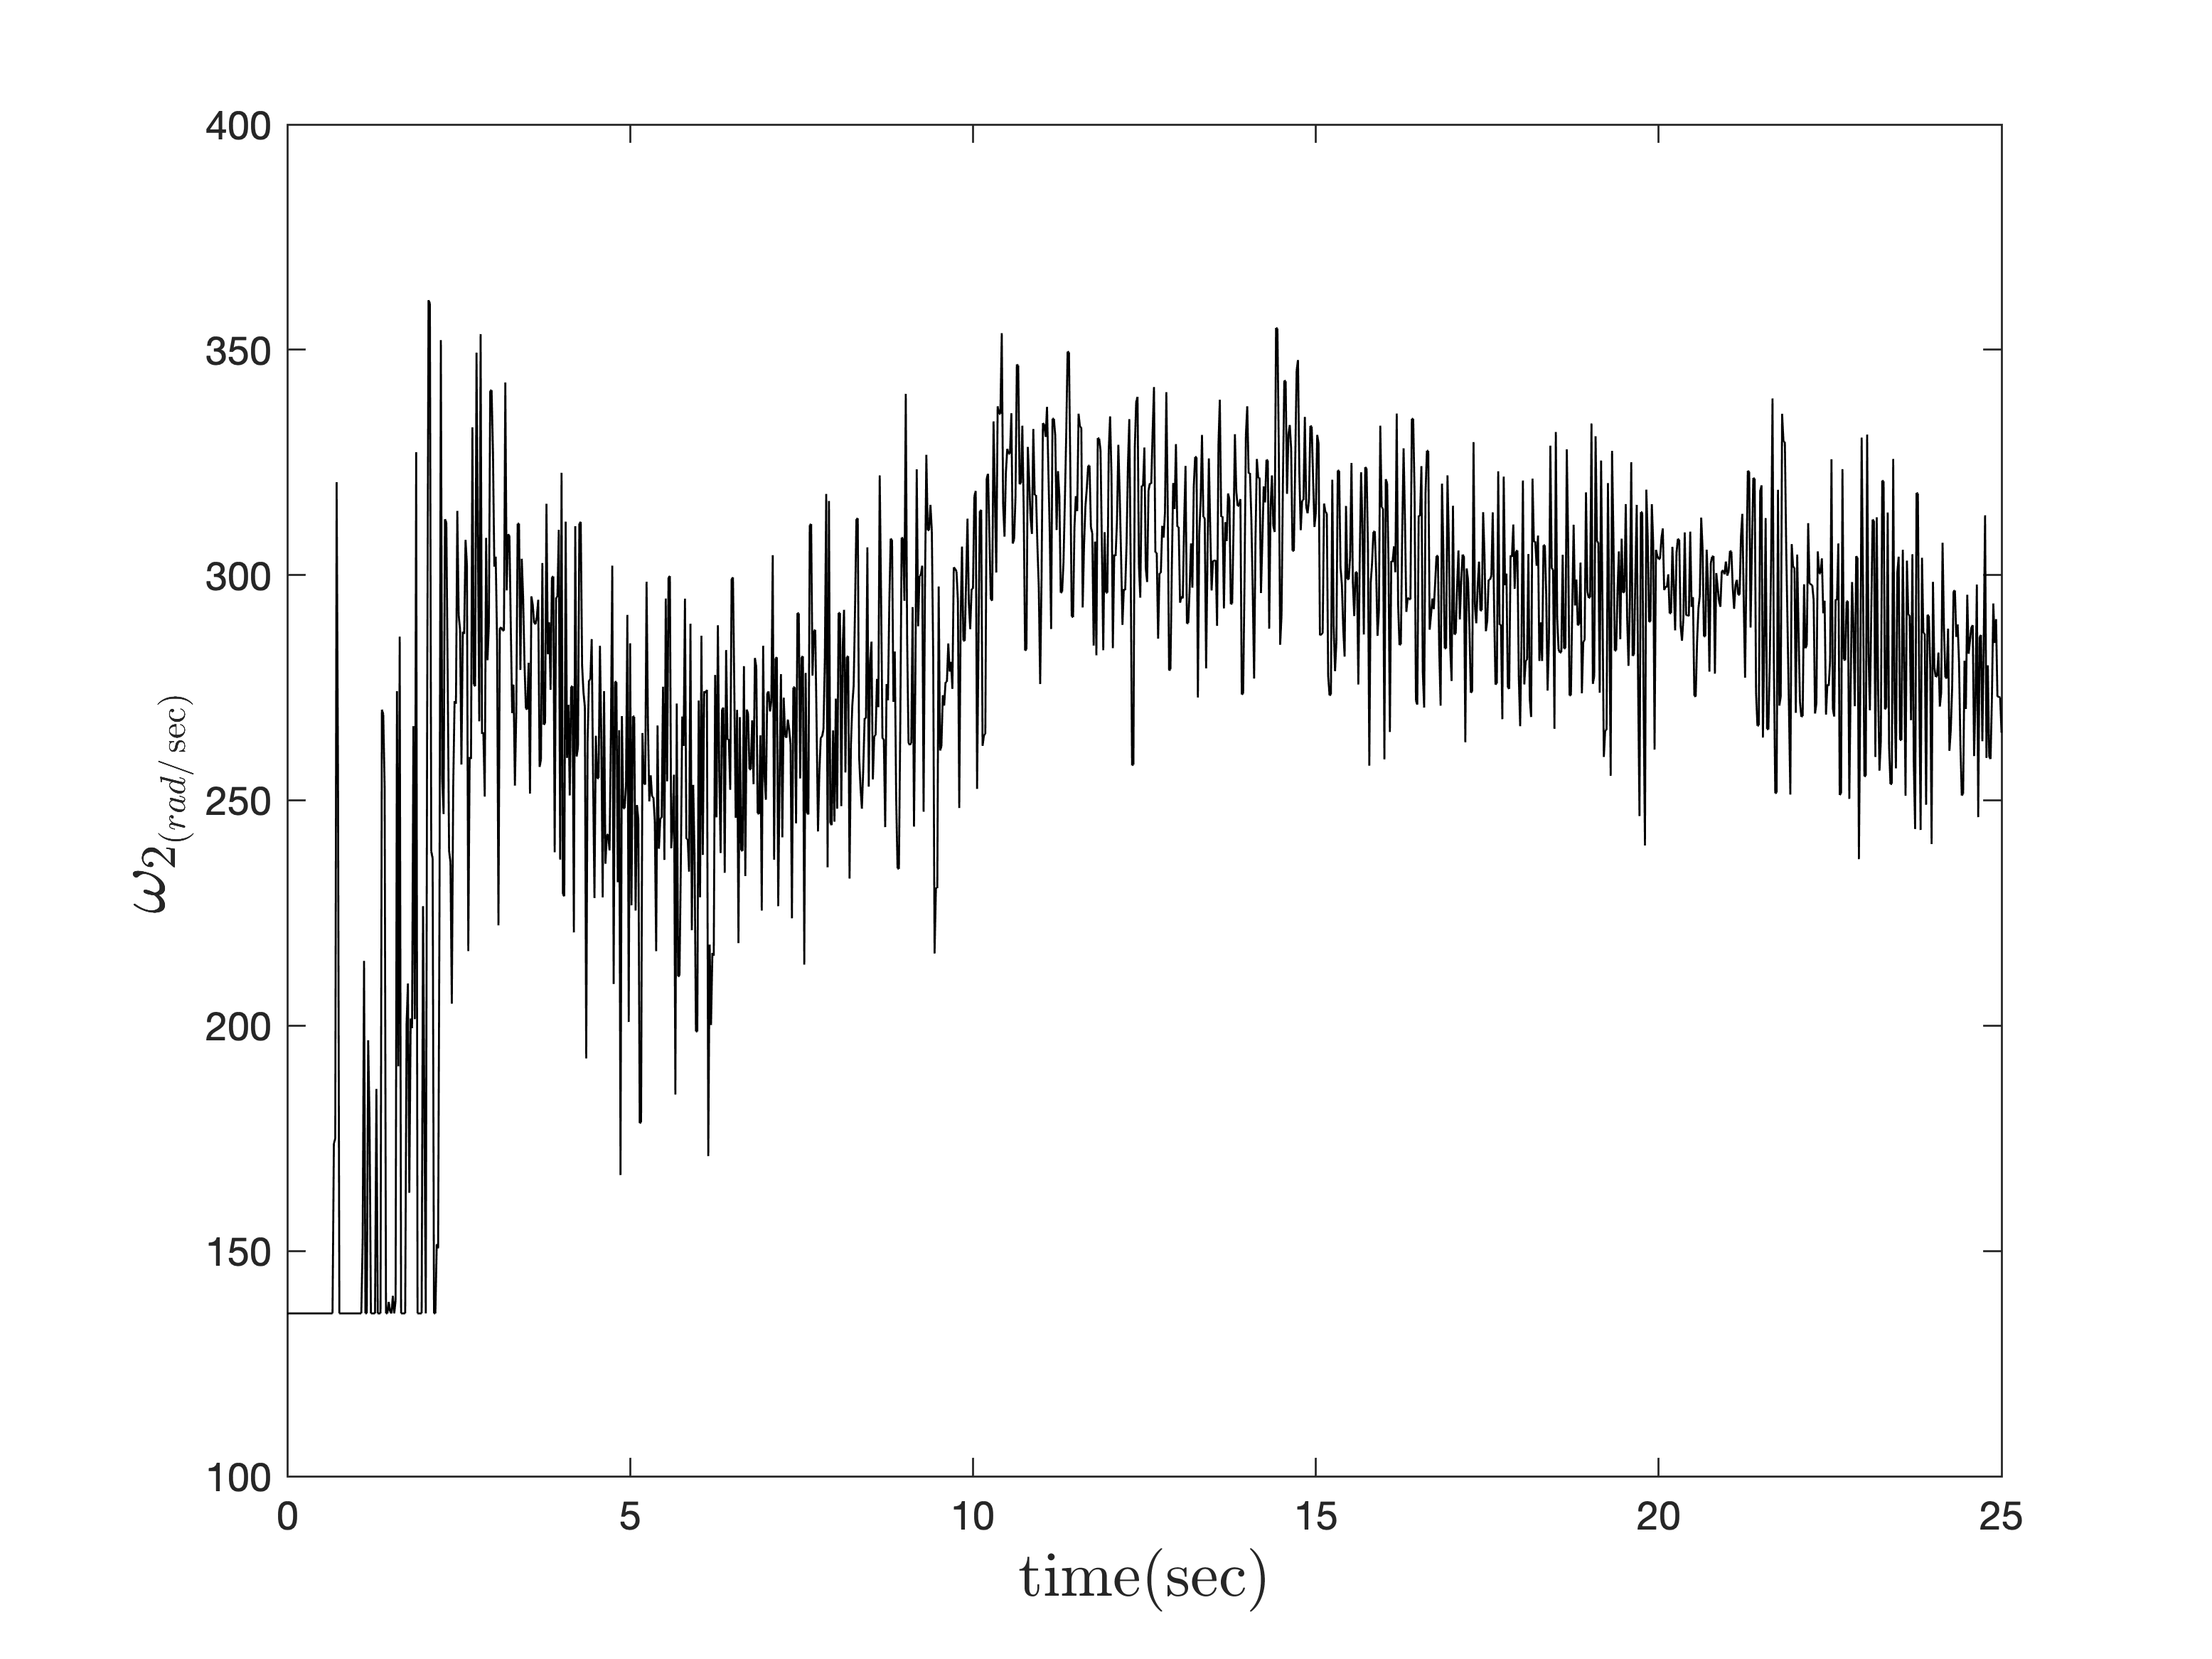
\includegraphics[width=.45\linewidth]{../Figures/Calibration/LQIDG/3DOF/lqidg_Omega_2.png}
	}
	\subfigure[موتور شماره سه]{
		\centering
		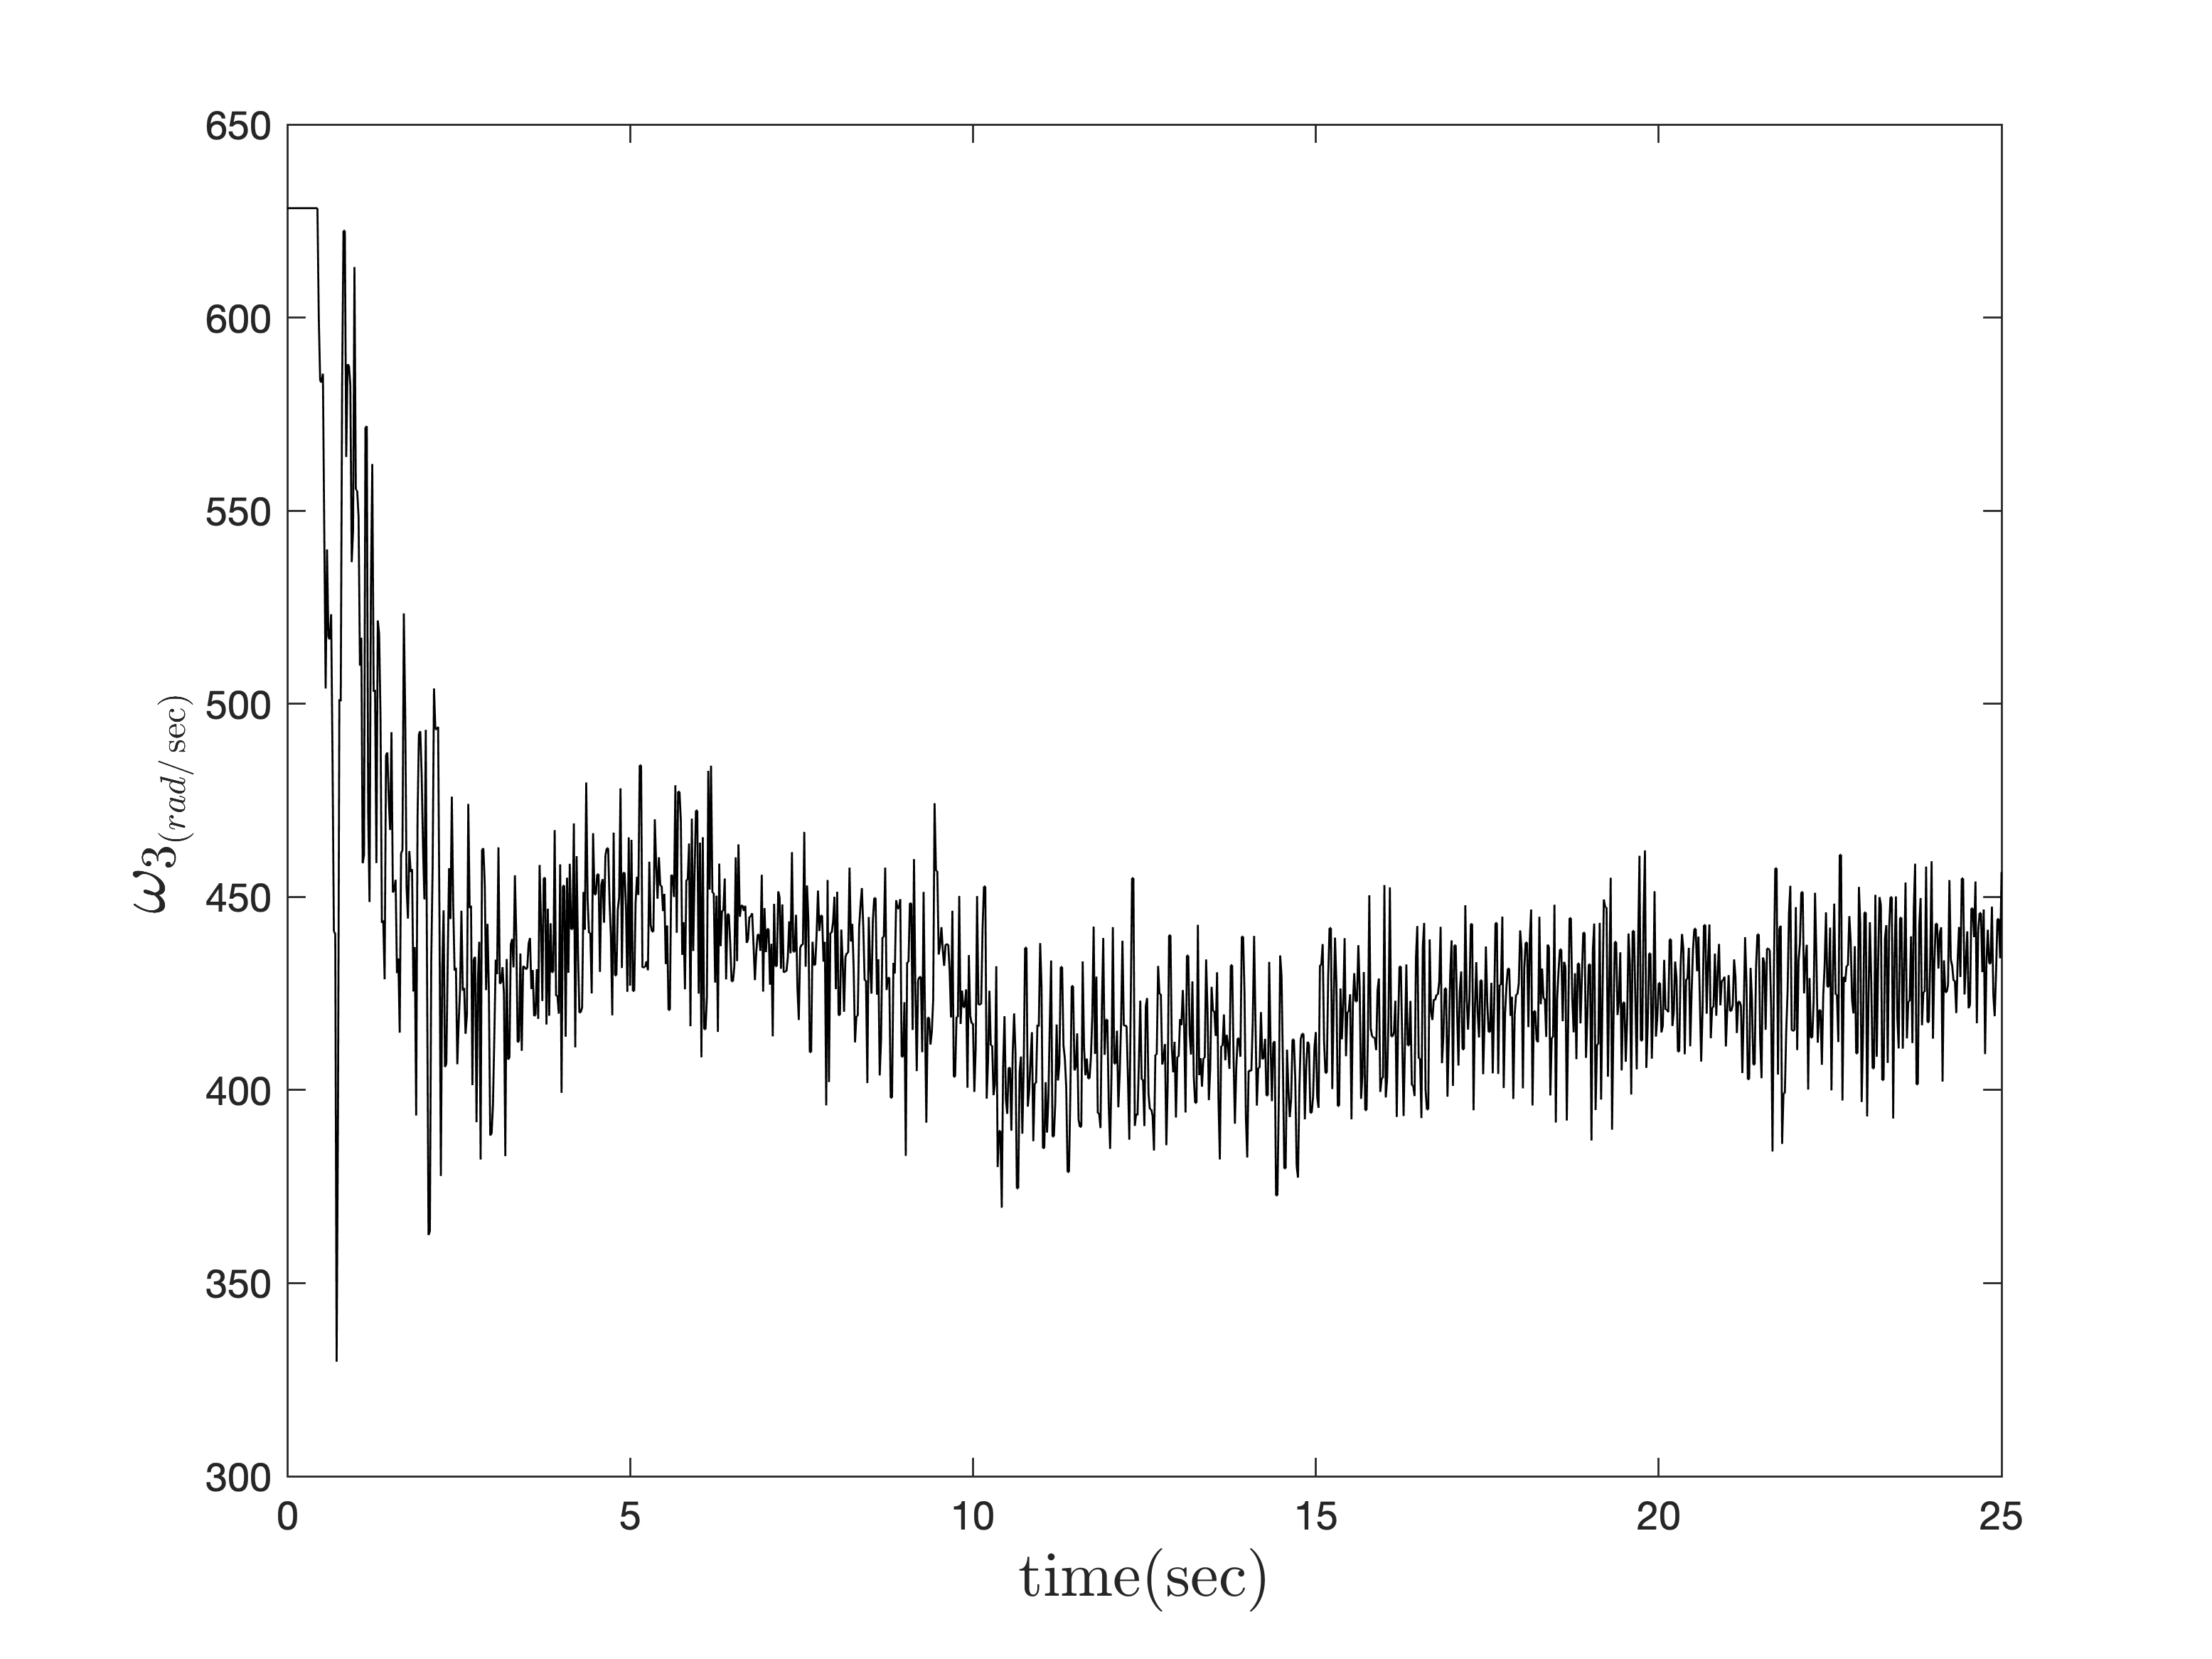
\includegraphics[width=.45\linewidth]{../Figures/Calibration/LQIDG/3DOF/lqidg_Omega_3.png}
	}
	\subfigure[موتور شماره چهار]{
		\centering
		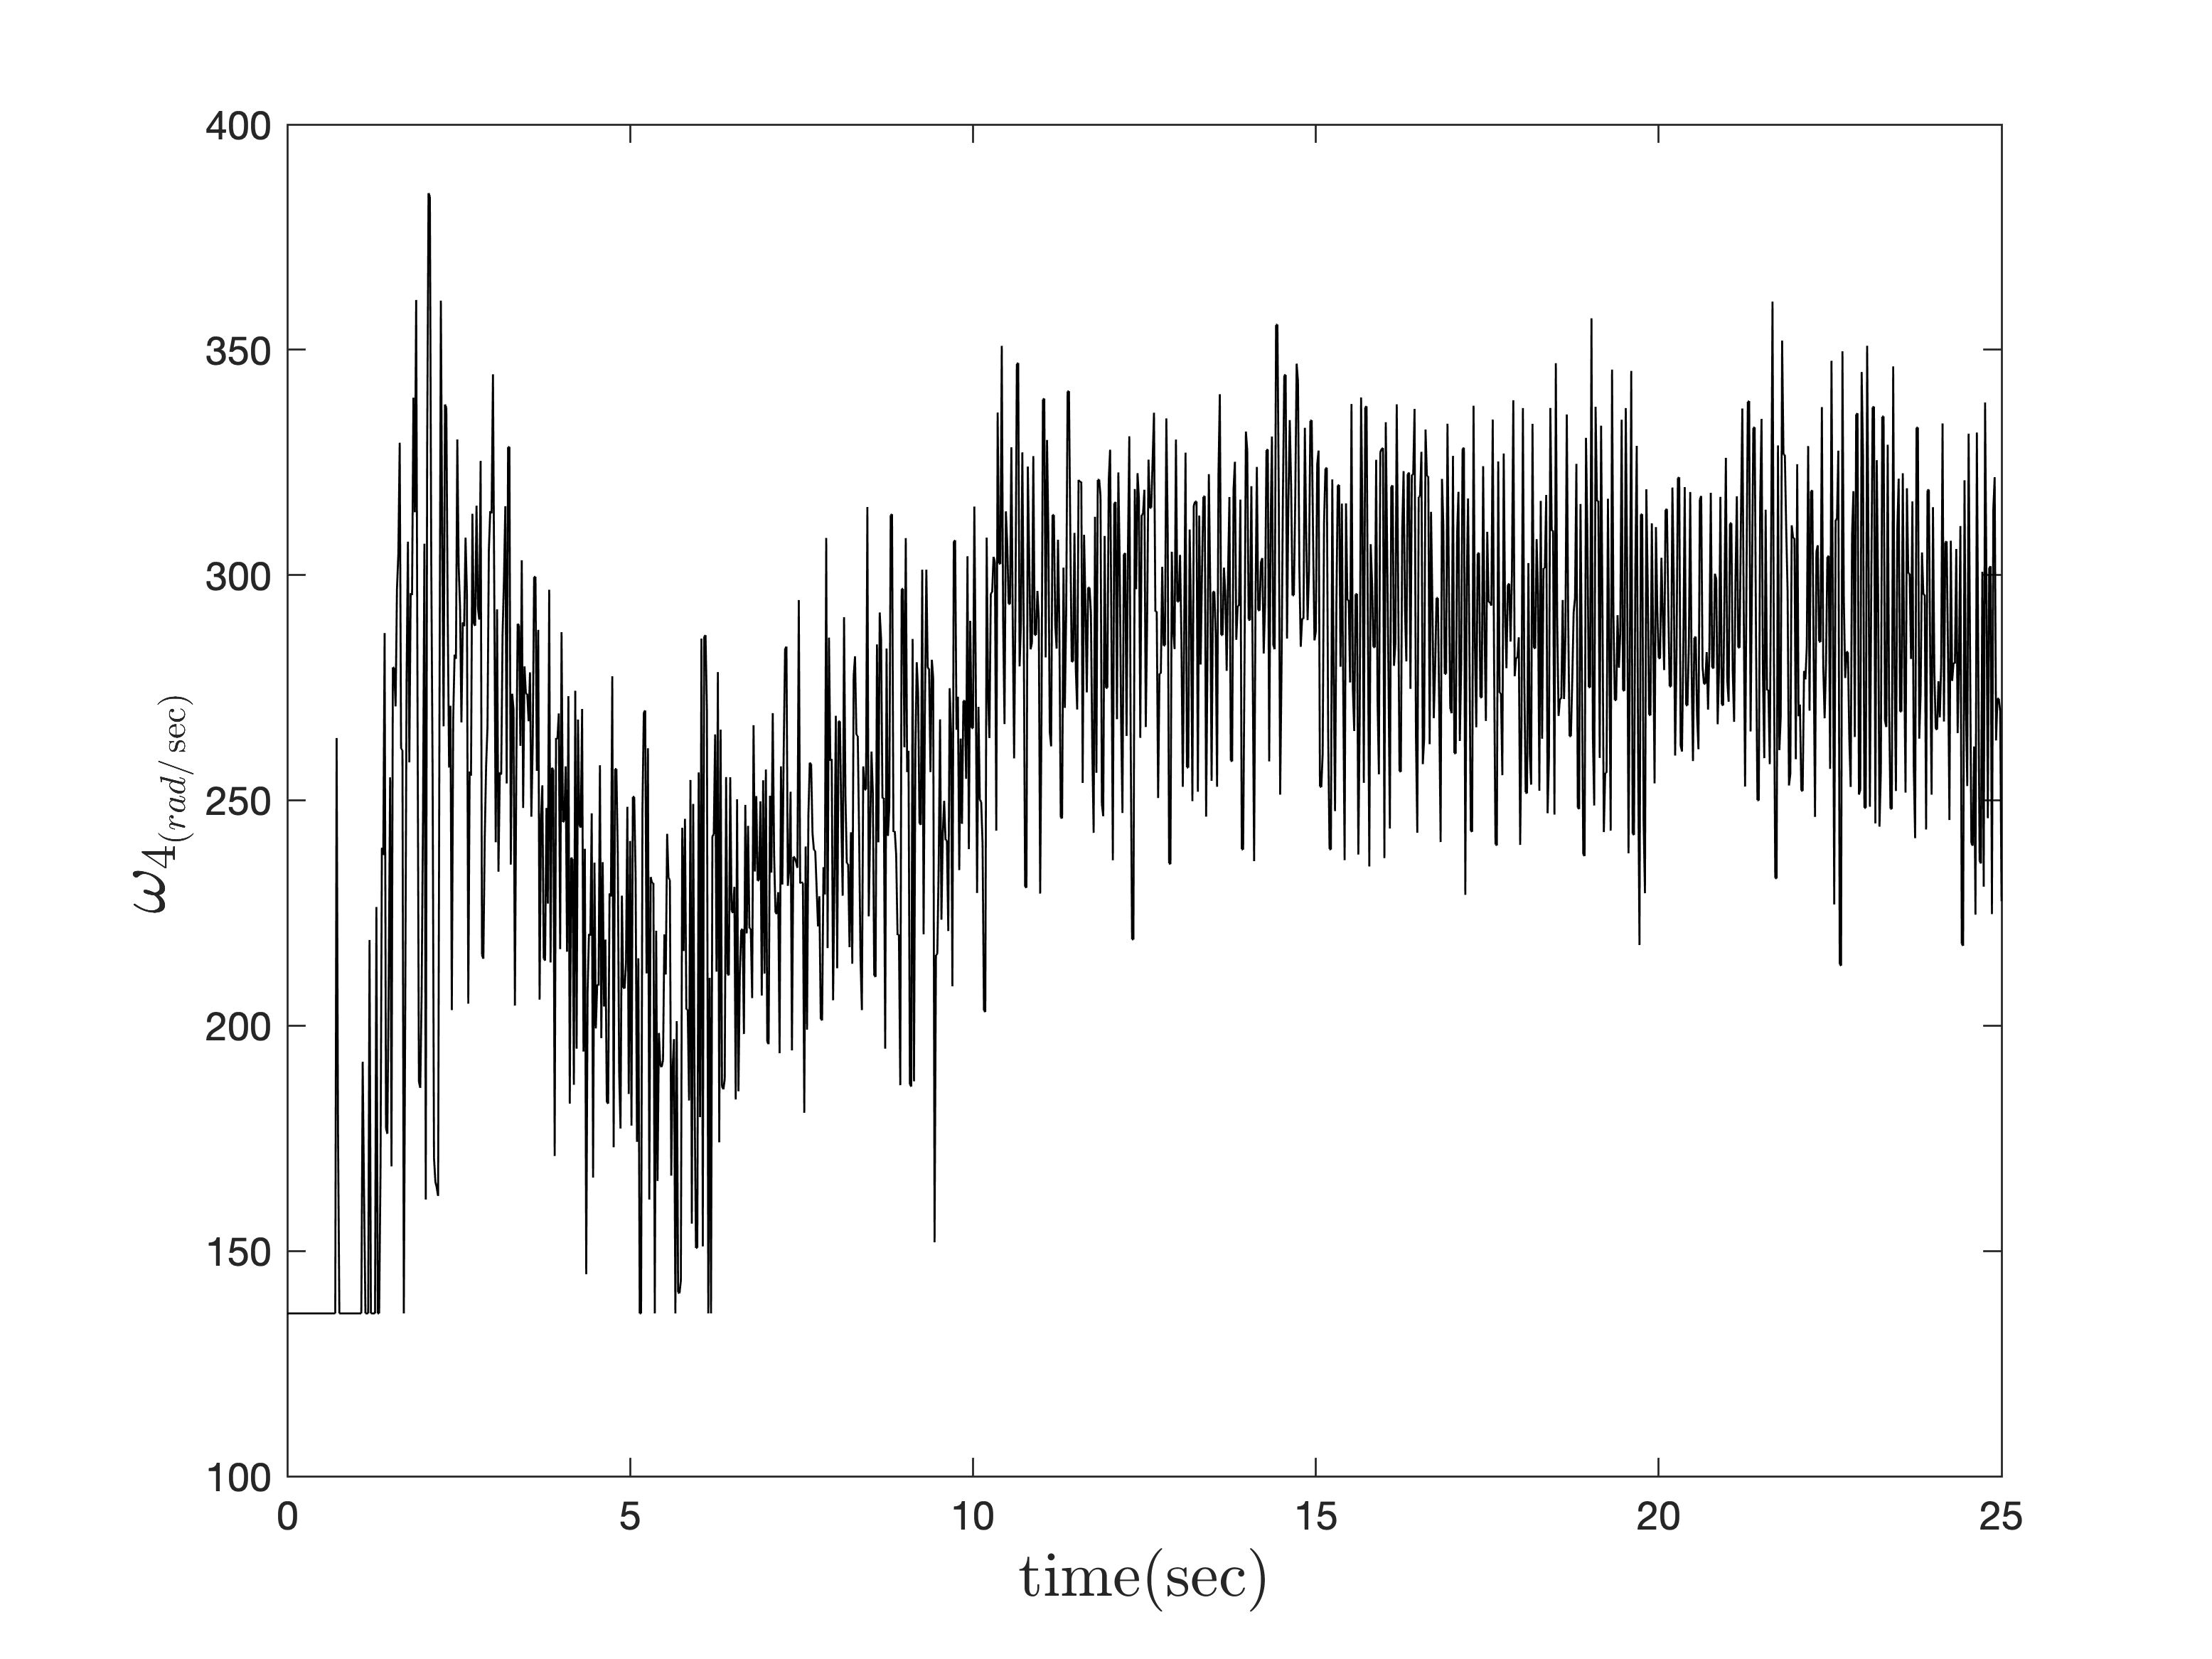
\includegraphics[width=.45\linewidth]{../Figures/Calibration/LQIDG/3DOF/lqidg_Omega_4.png}
	}
	\caption{‫‪فرمان کنترلی موتورها در کنترل وضعیت (تعقیب ورودی صفر)}
\end{figure}

\subsection{پیاده‌سازی کنترل‌کننده به‌صورت چهار ورودی}\label{lqidg_mimo}


\begin{figure}[H]
	\centering
	\subfigure[تغییرات زاویه رول]{
		\centering
		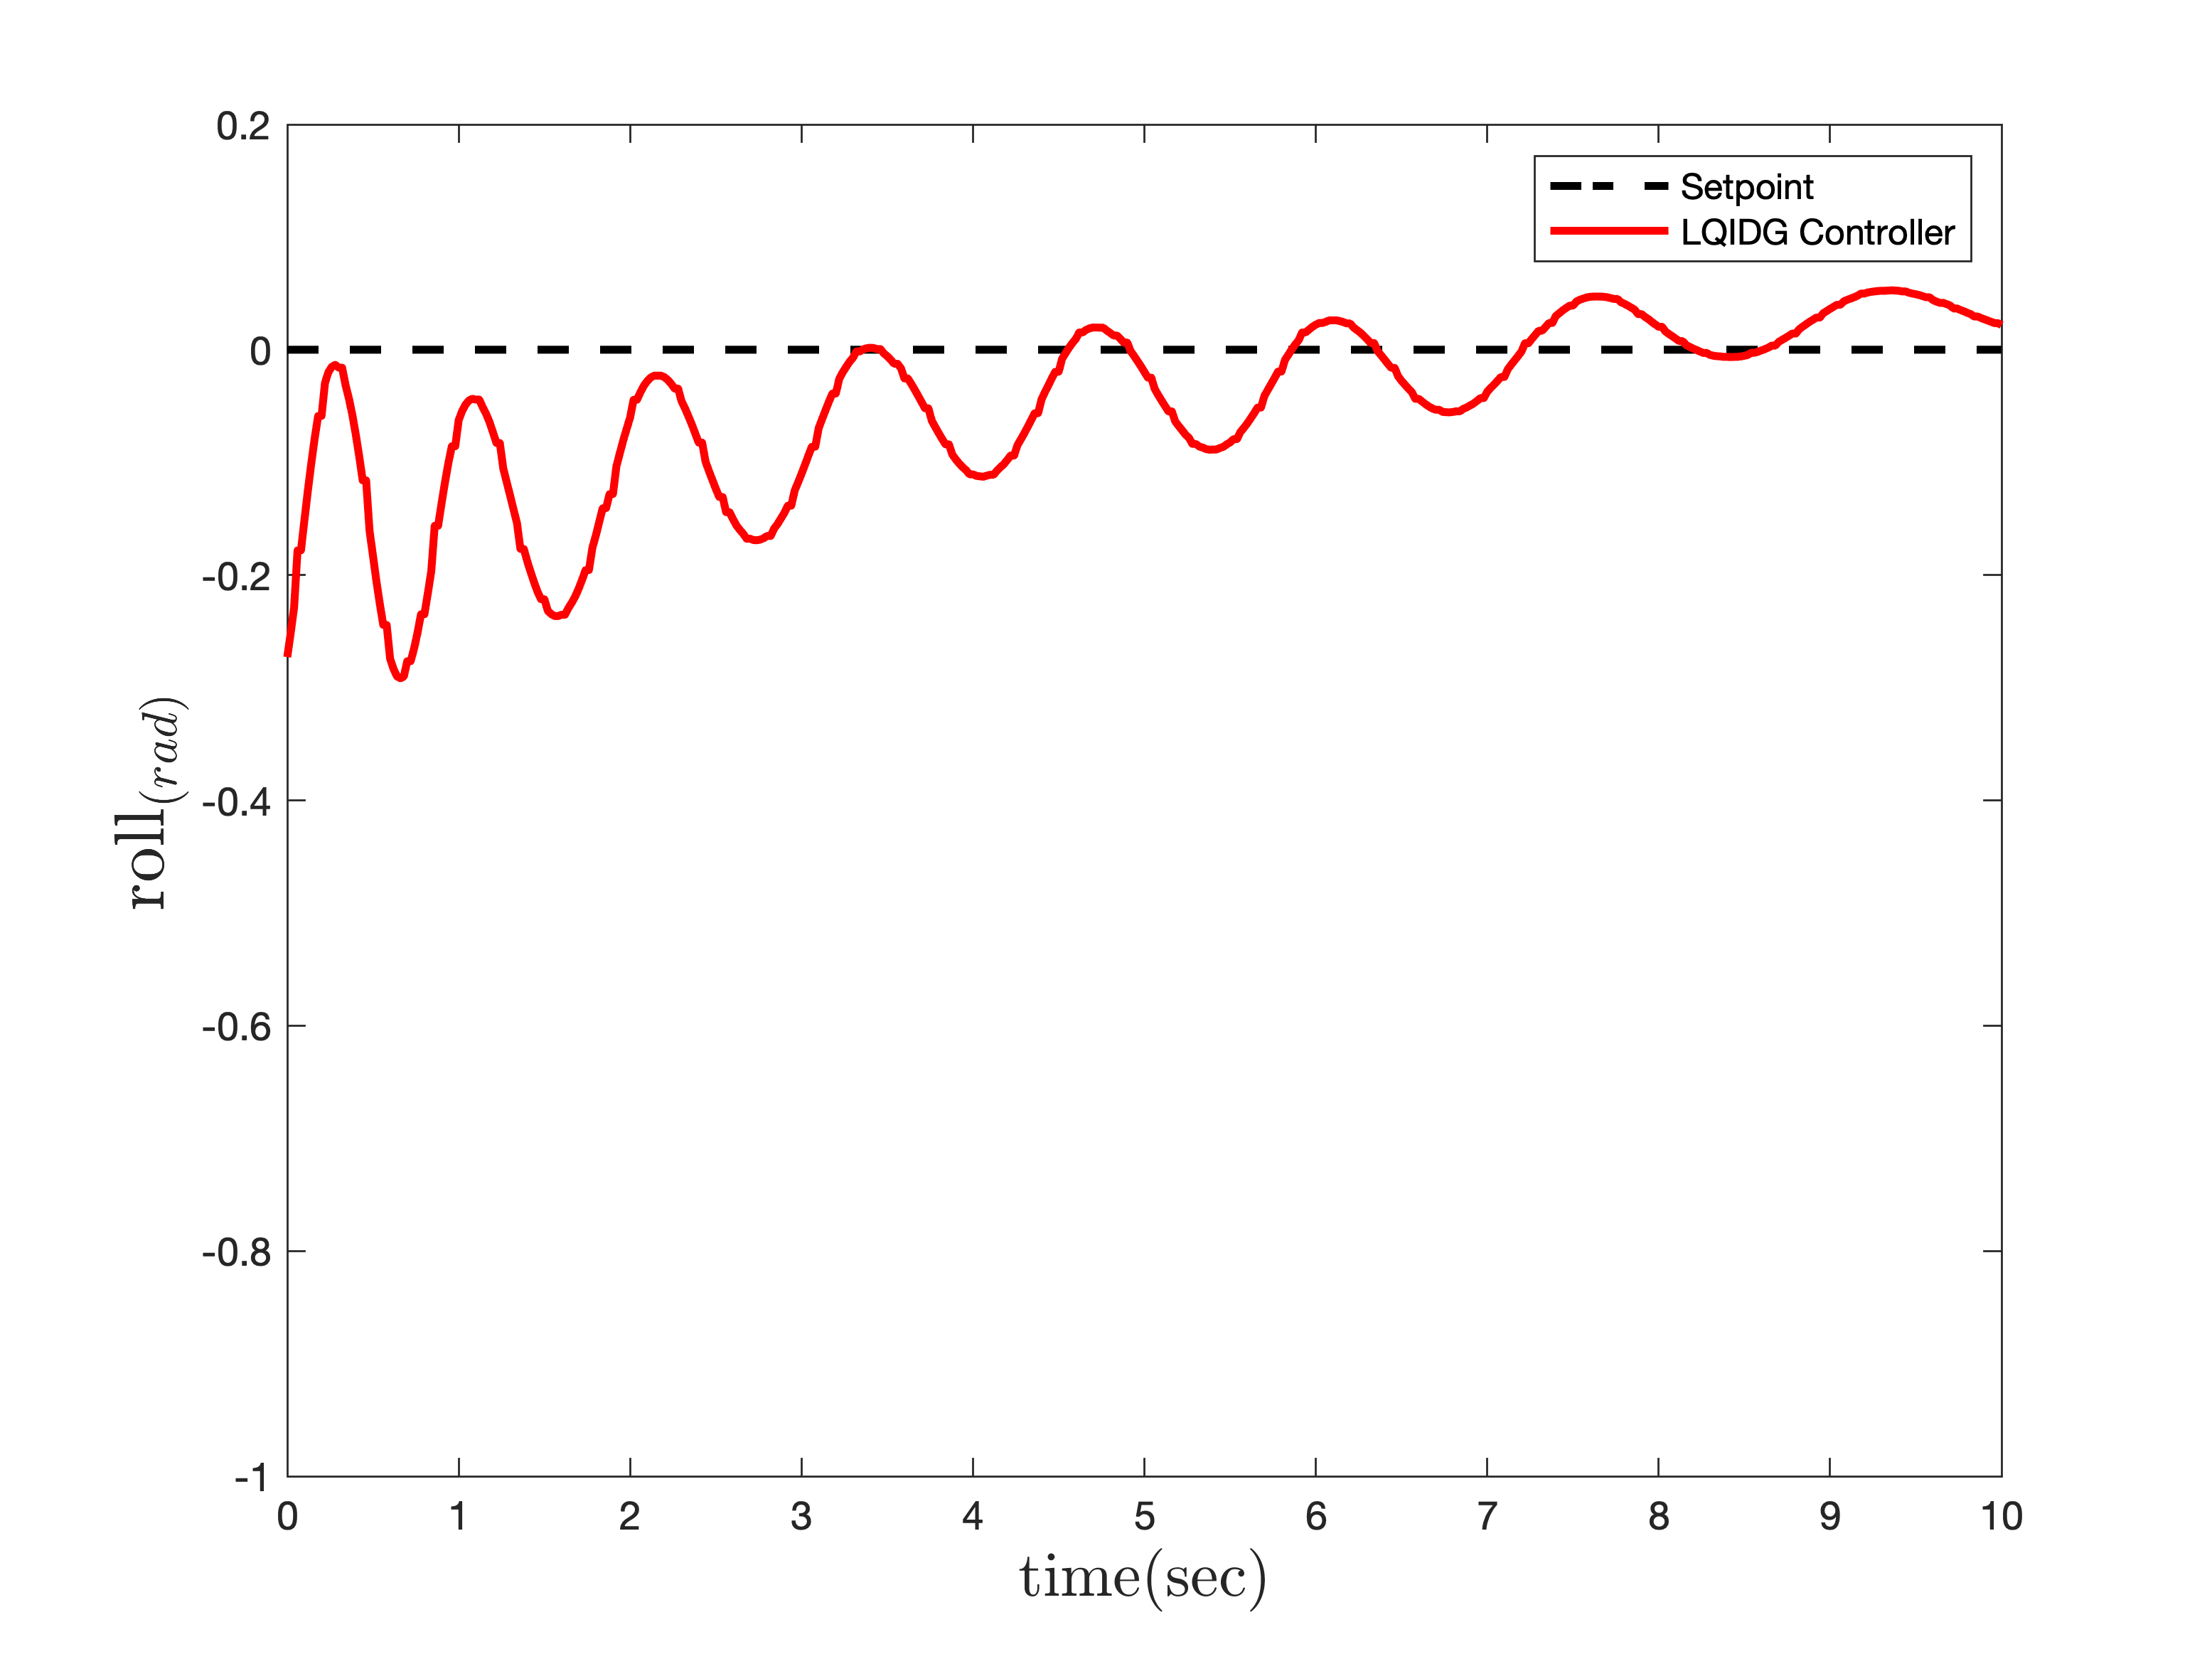
\includegraphics[width=.48\linewidth]{../Figures/Calibration/LQIDG/MIMO/lqidg_roll.png}
	}
	\subfigure[تغییرات زاویه پیچ]{
		\centering
		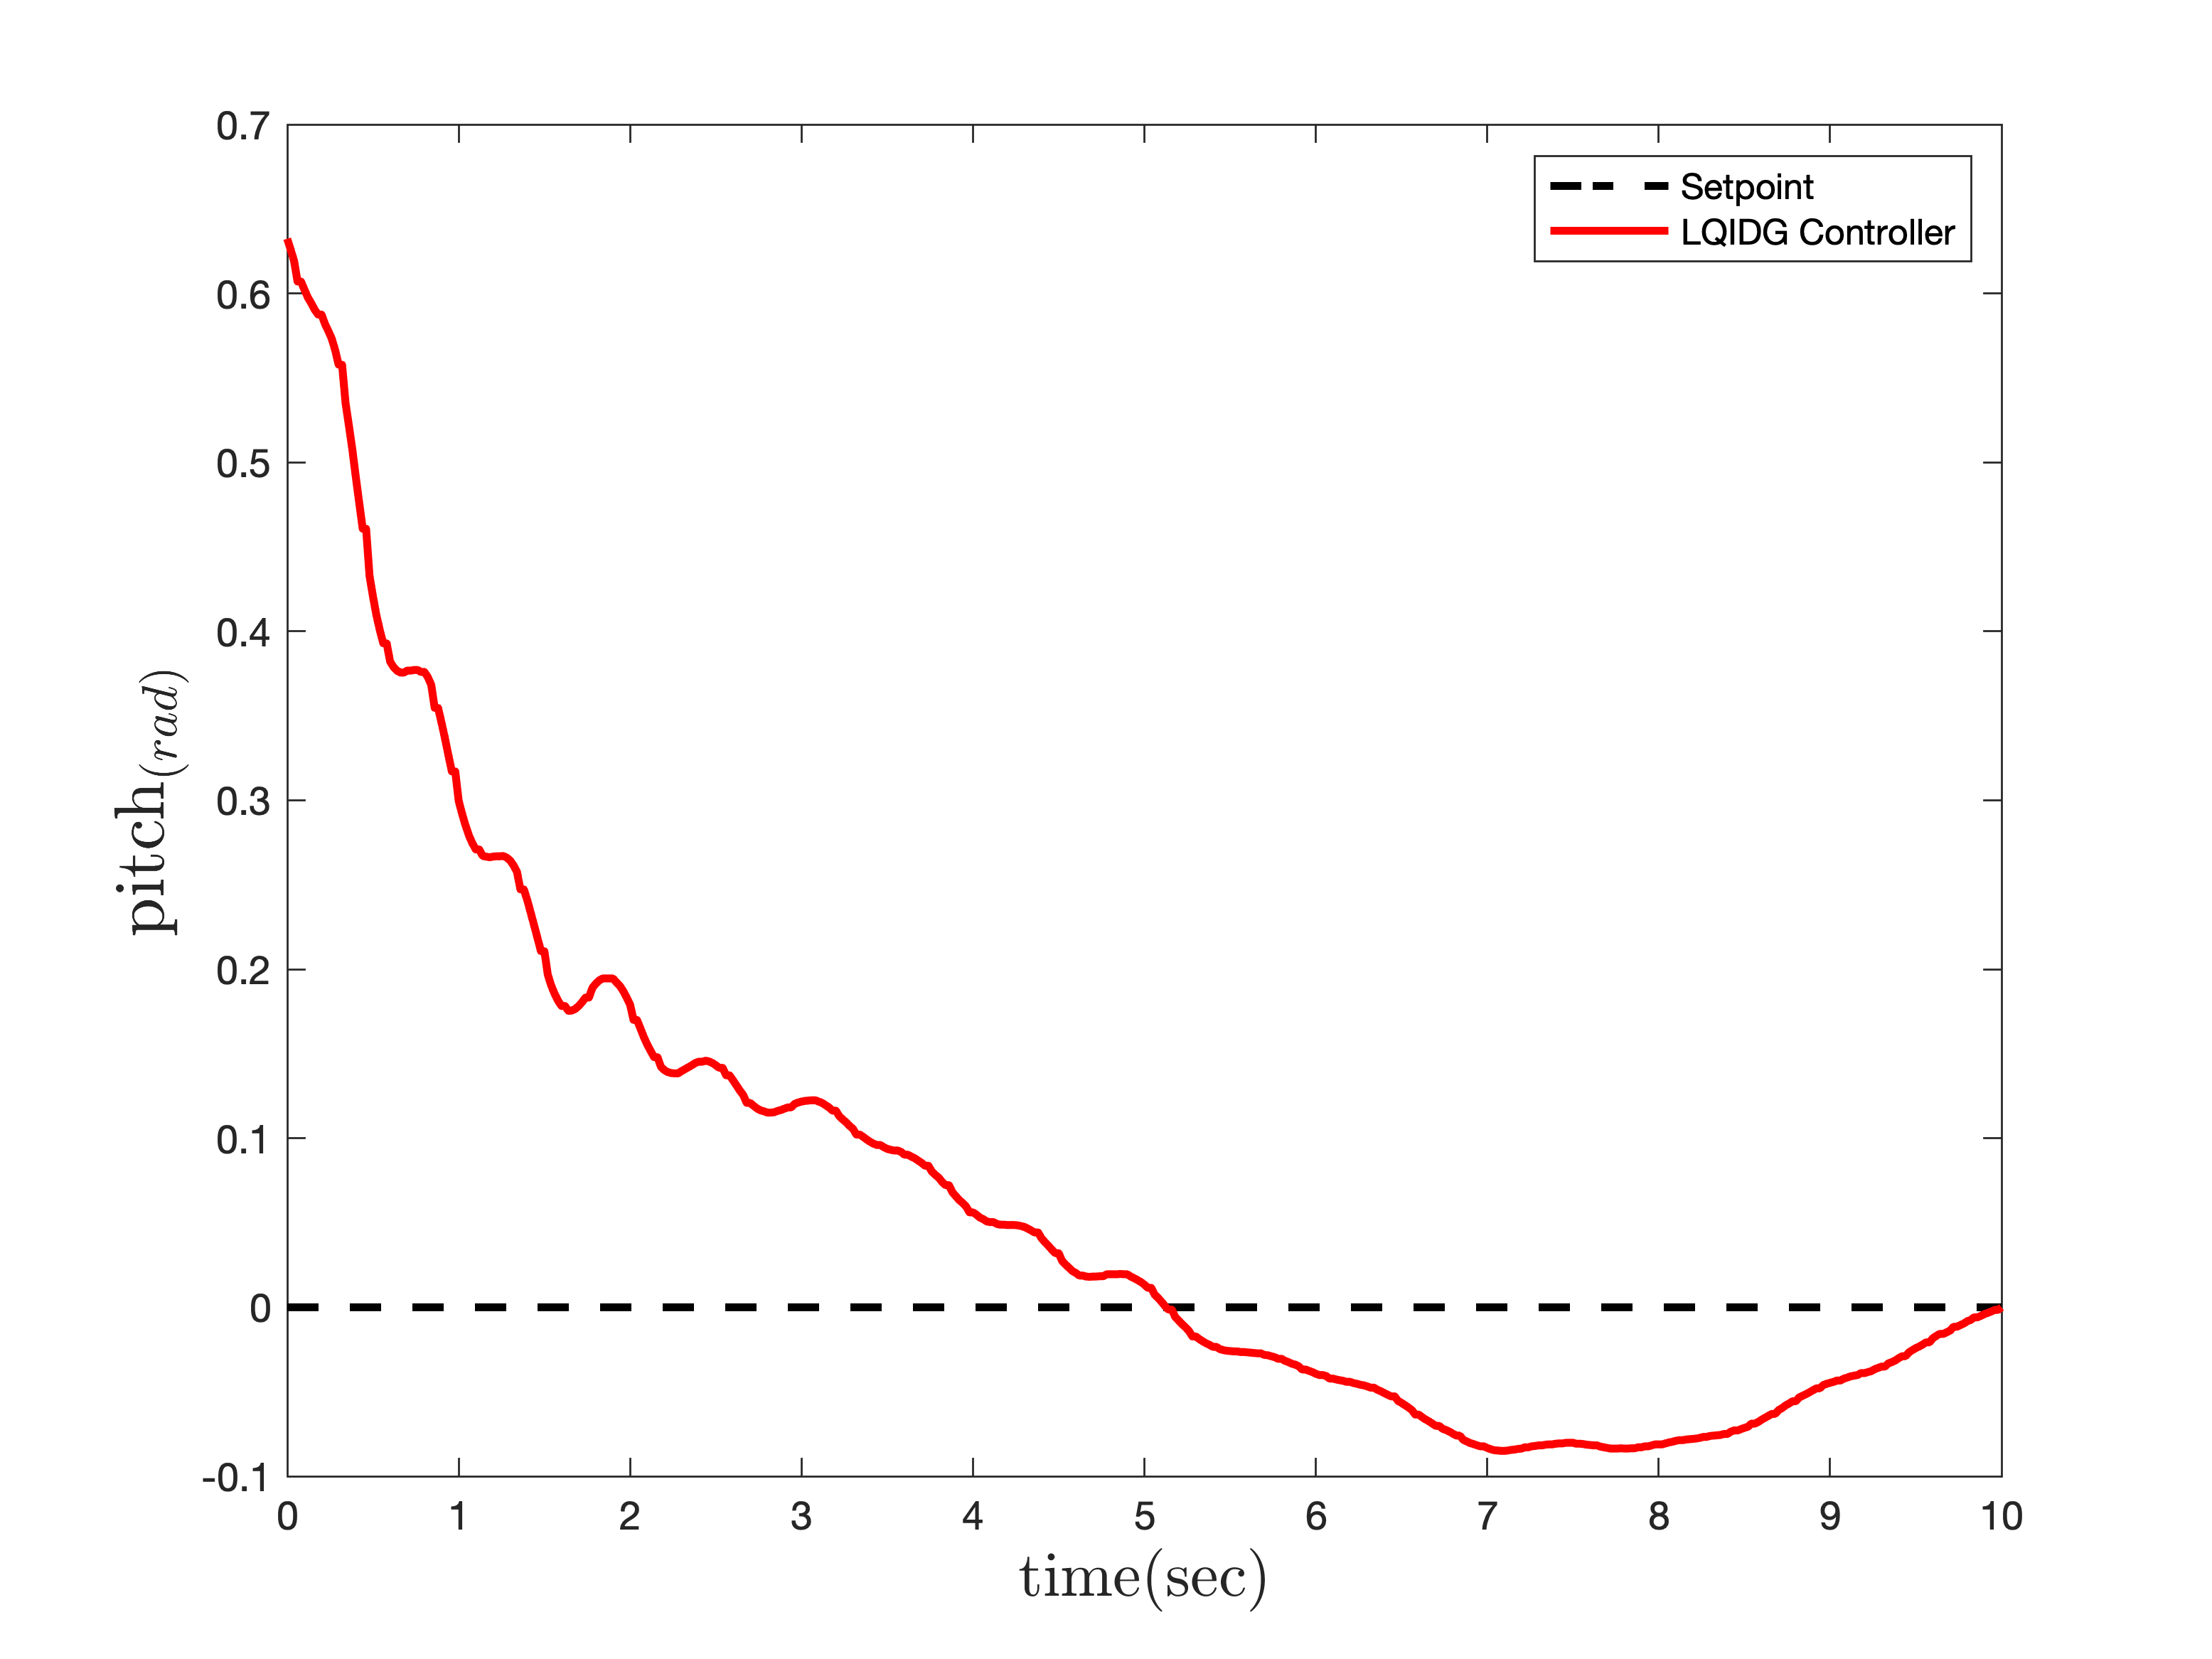
\includegraphics[width=.48\linewidth]{../Figures/Calibration/LQIDG/MIMO/lqidg_pitch.png}
	}
	\subfigure[تغییرات زاویه یاو]{
		\centering
		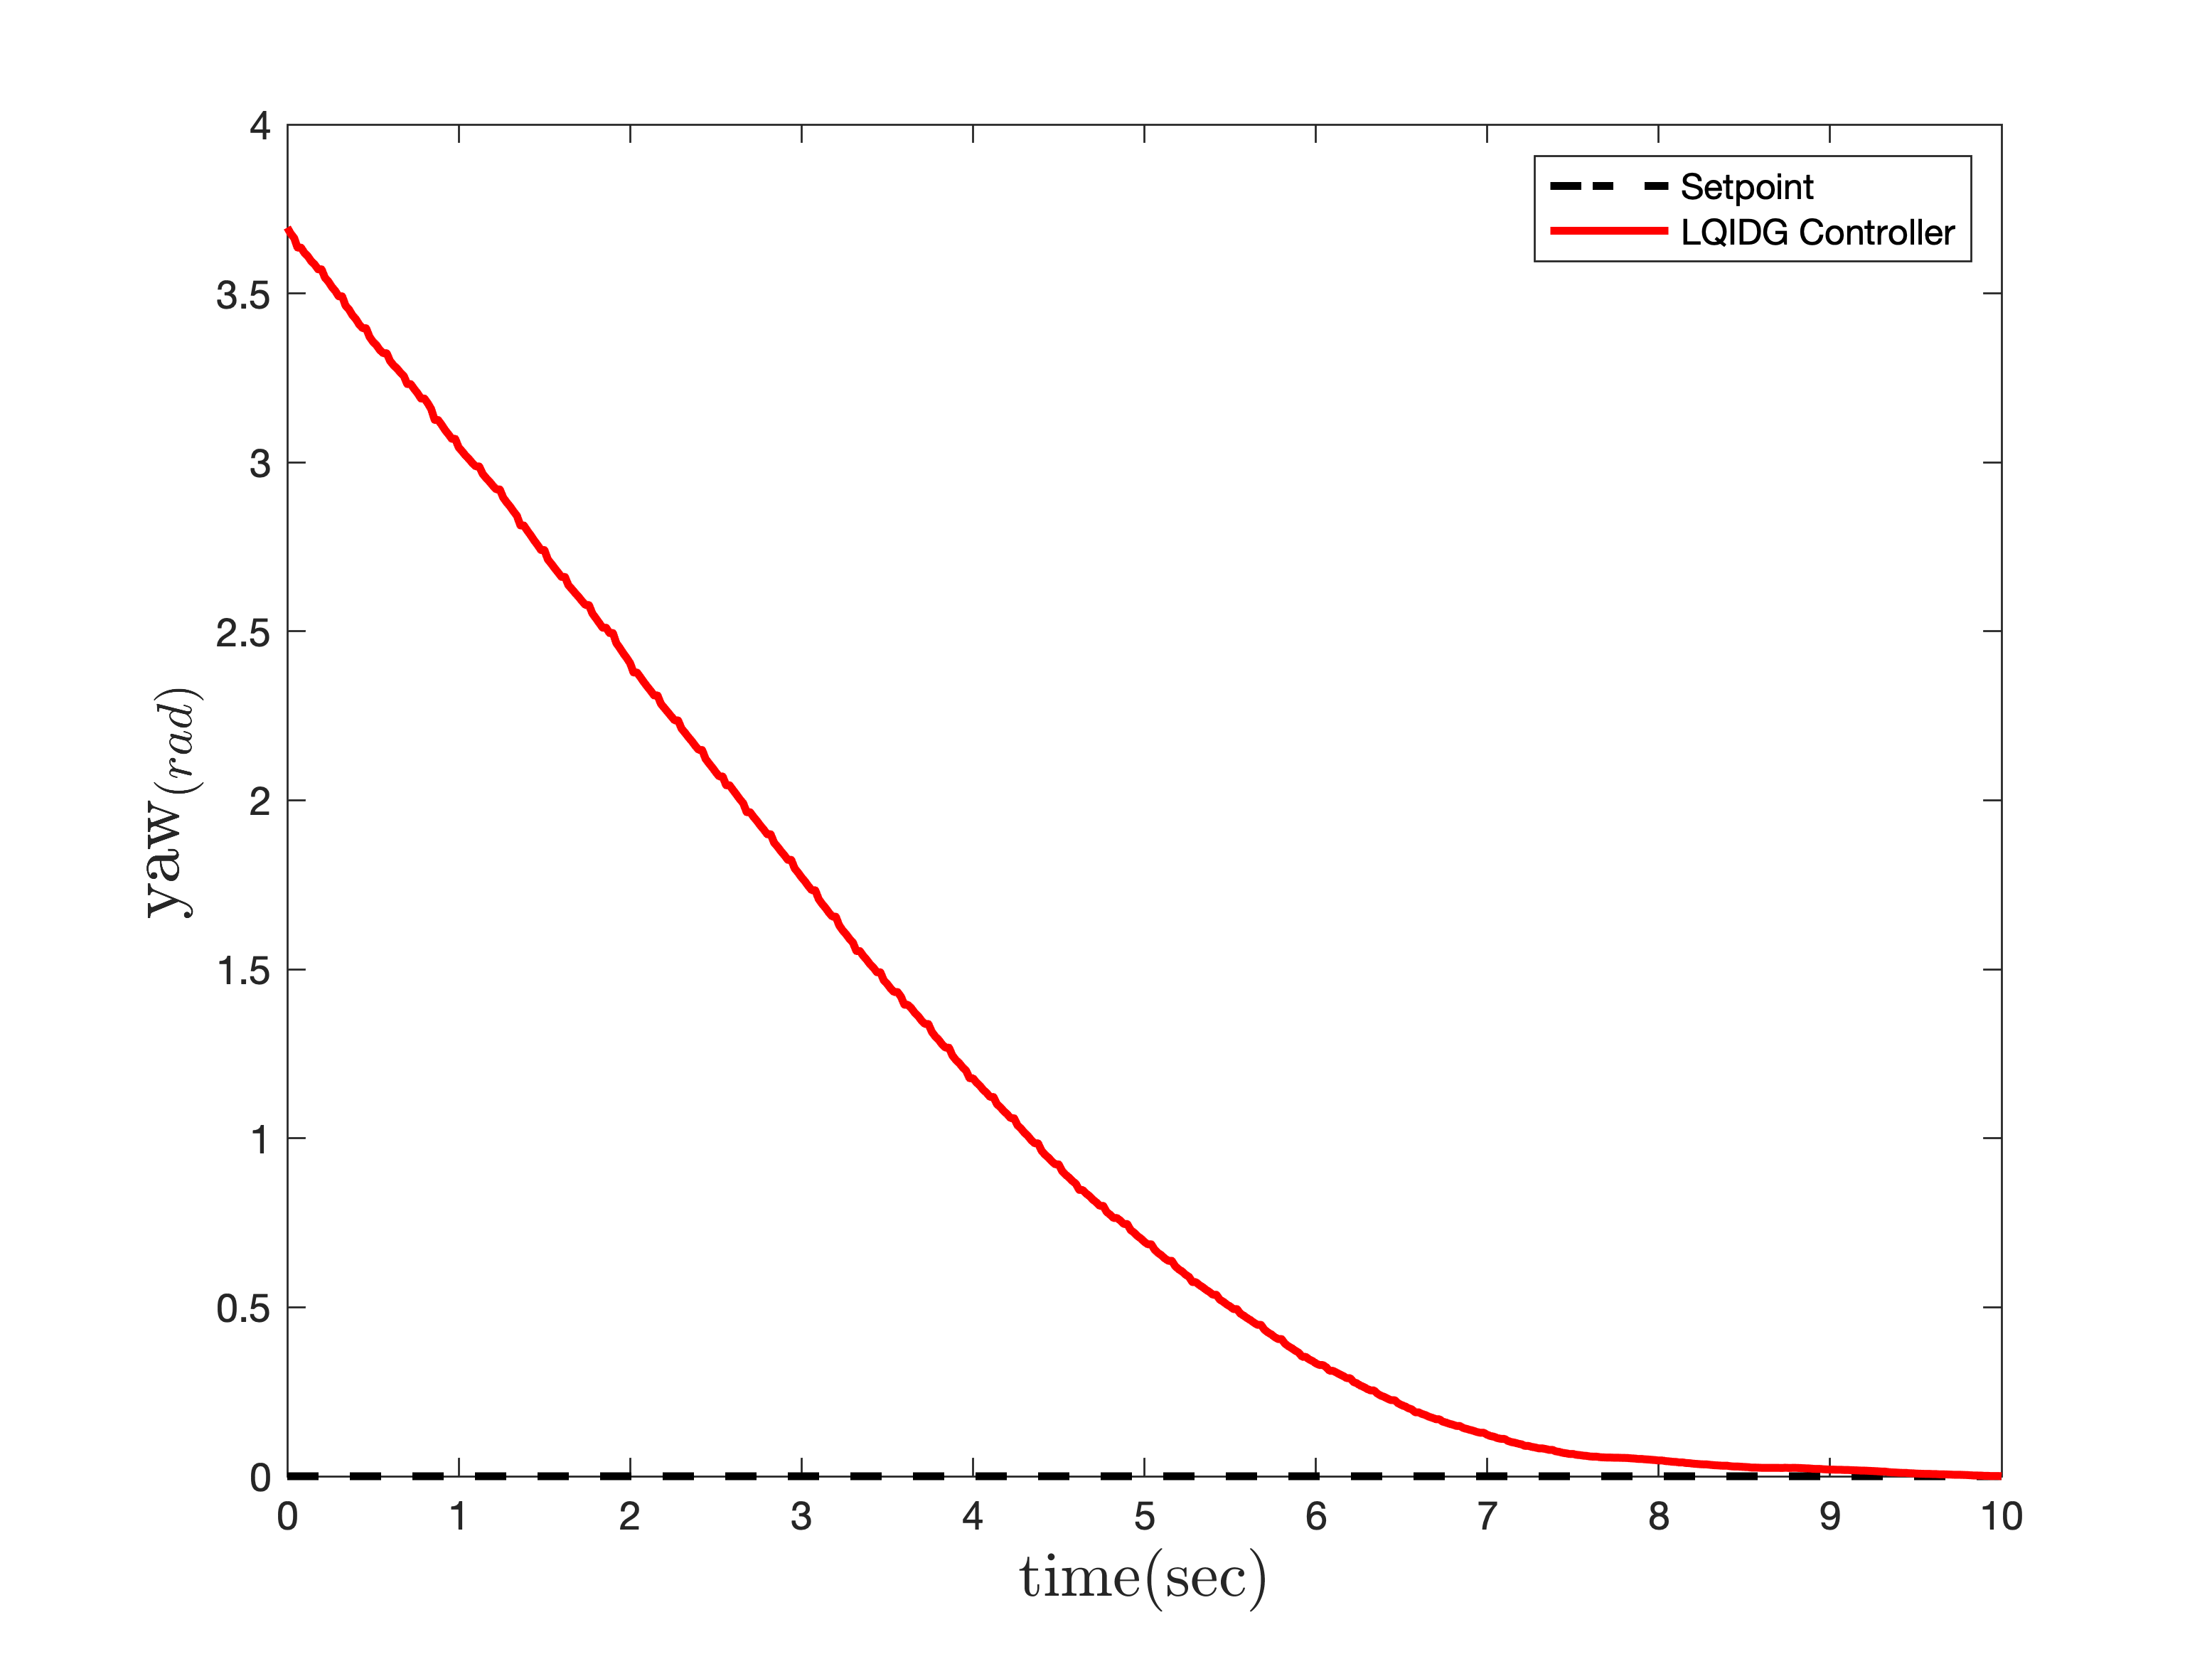
\includegraphics[width=.48\linewidth]{../Figures/Calibration/LQIDG/MIMO/lqidg_yaw.png}
	}
	\caption{‫‪عملکرد کنترل‌کننده \lr{LQIDG} در کنترل وضعیت (تعقیب ورودی صفر)}
\end{figure}



\begin{figure}[H]
	\centering
	\subfigure[موتور شماره یک]{
		\centering
		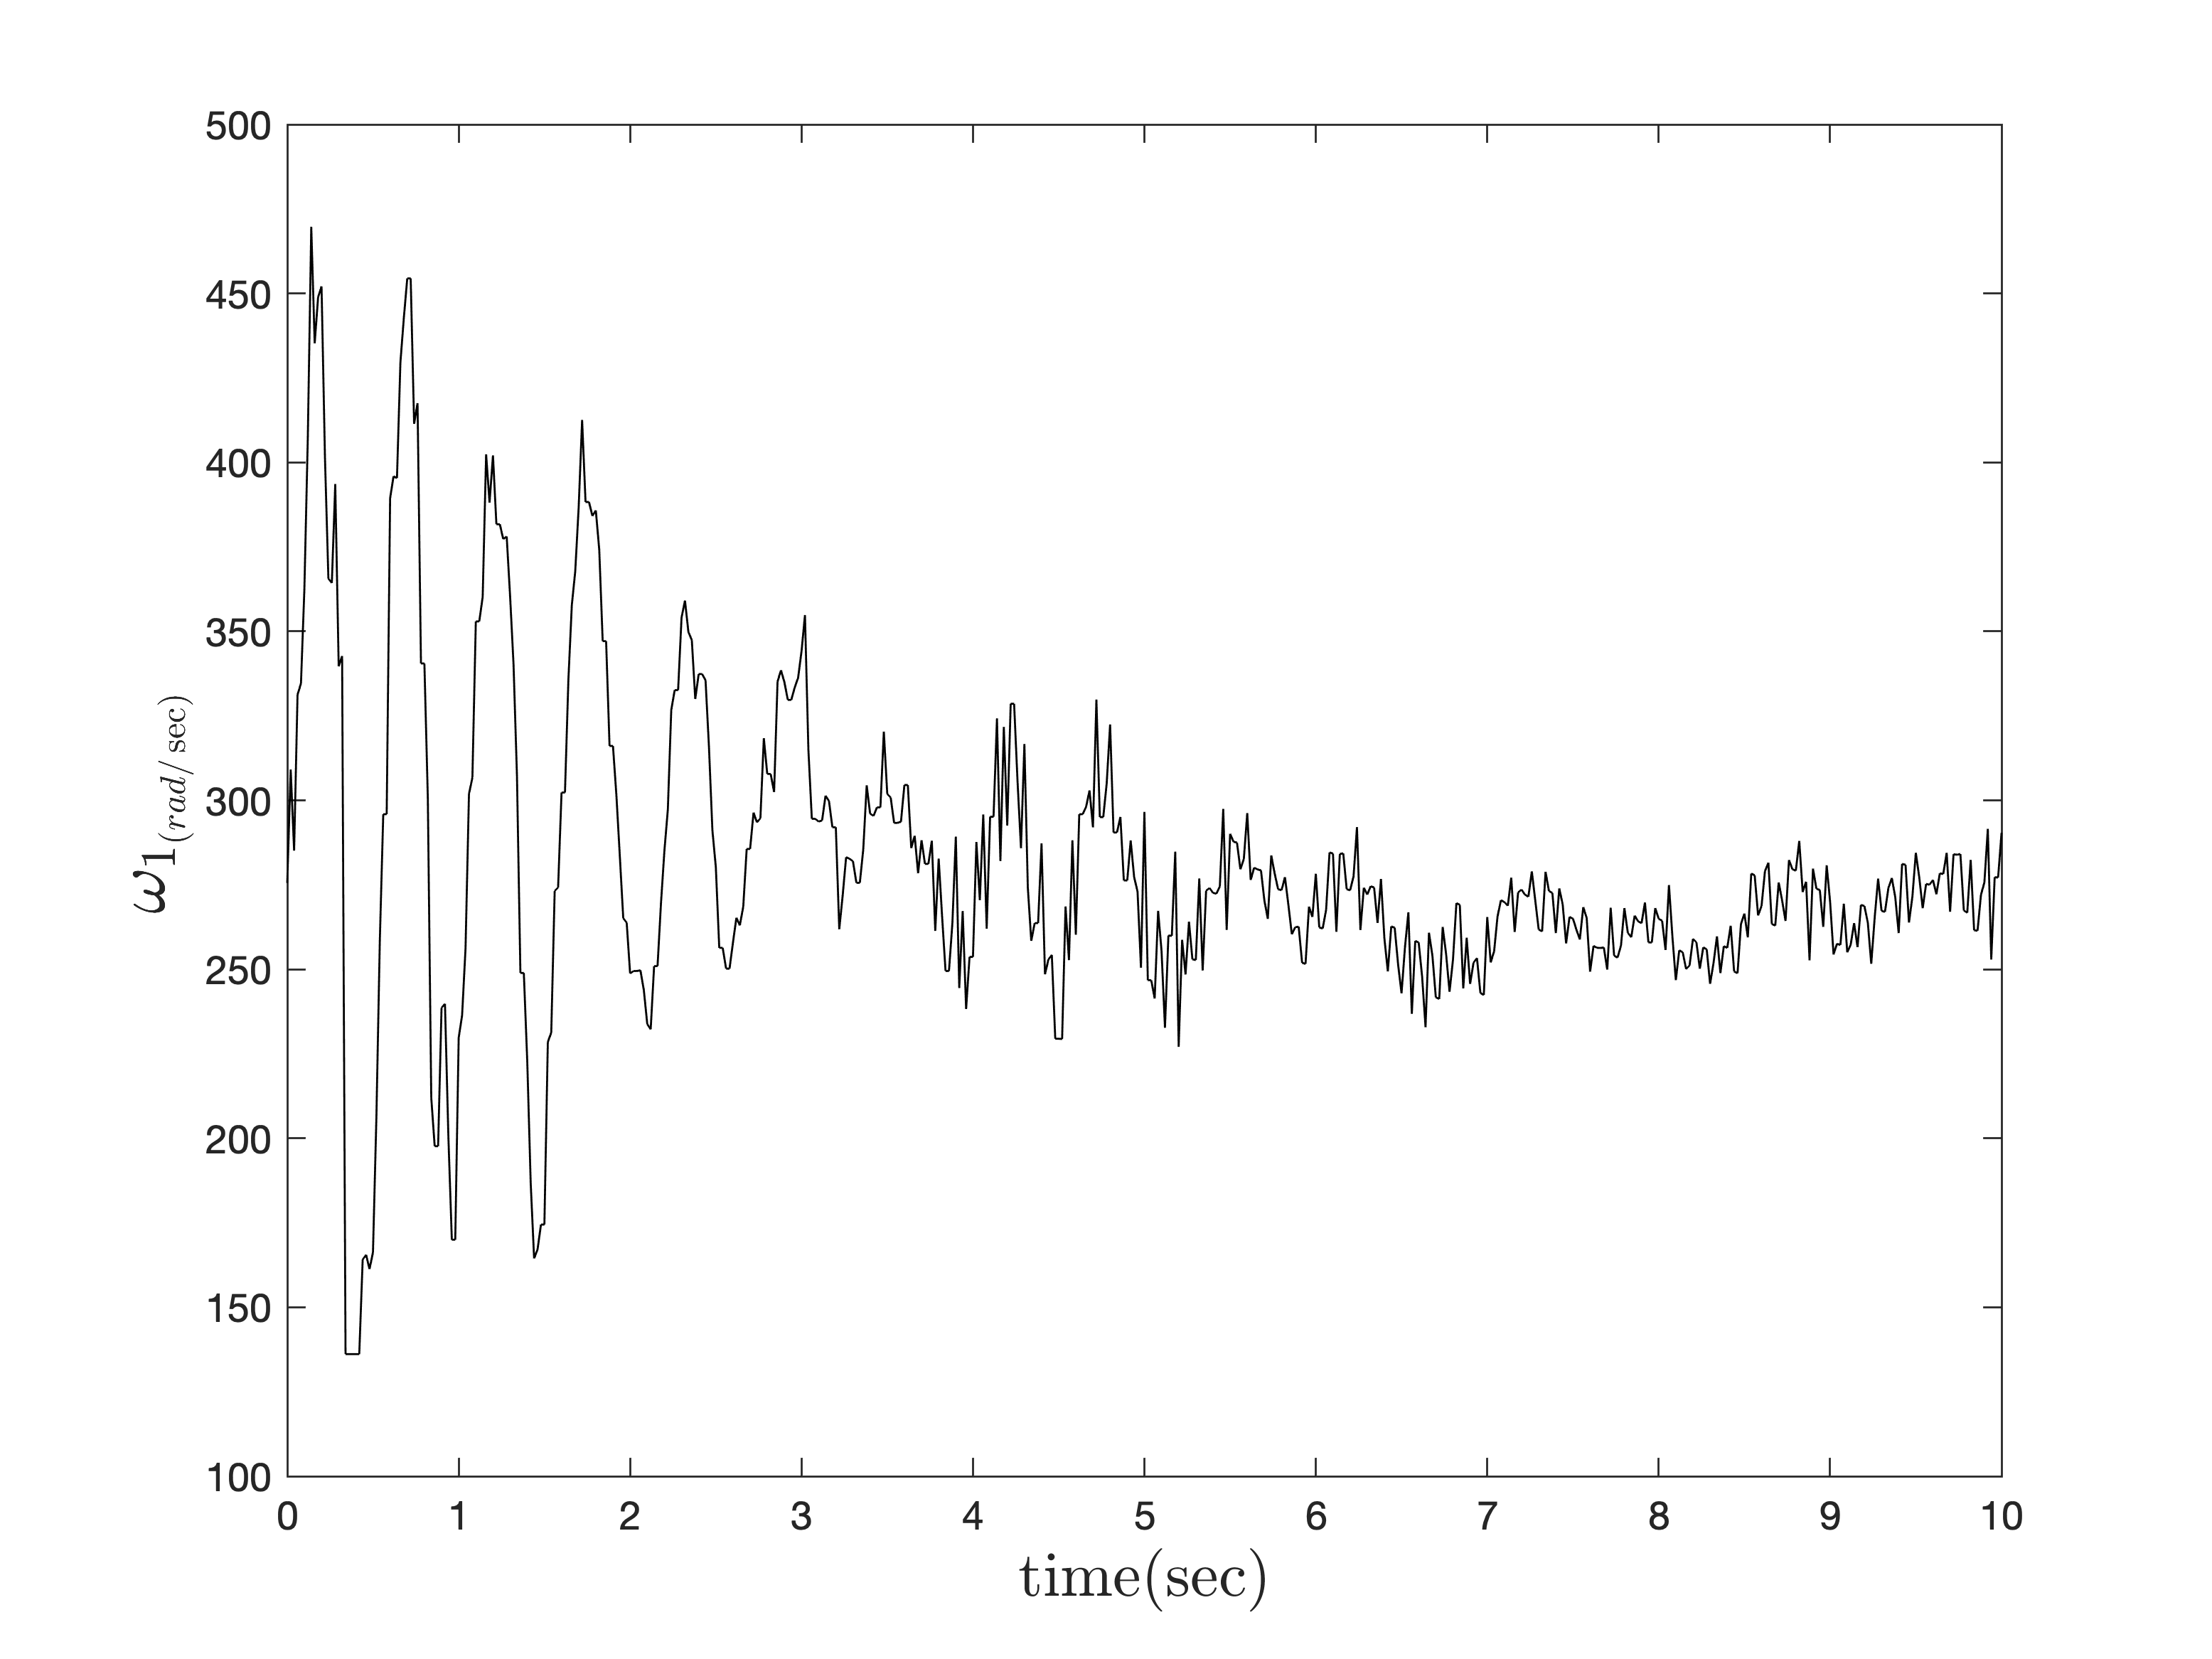
\includegraphics[width=.45\linewidth]{../Figures/Calibration/LQIDG/MIMO/lqidg_Omega_1.png}
	}
	\subfigure[موتور شماره دو]{
		\centering
		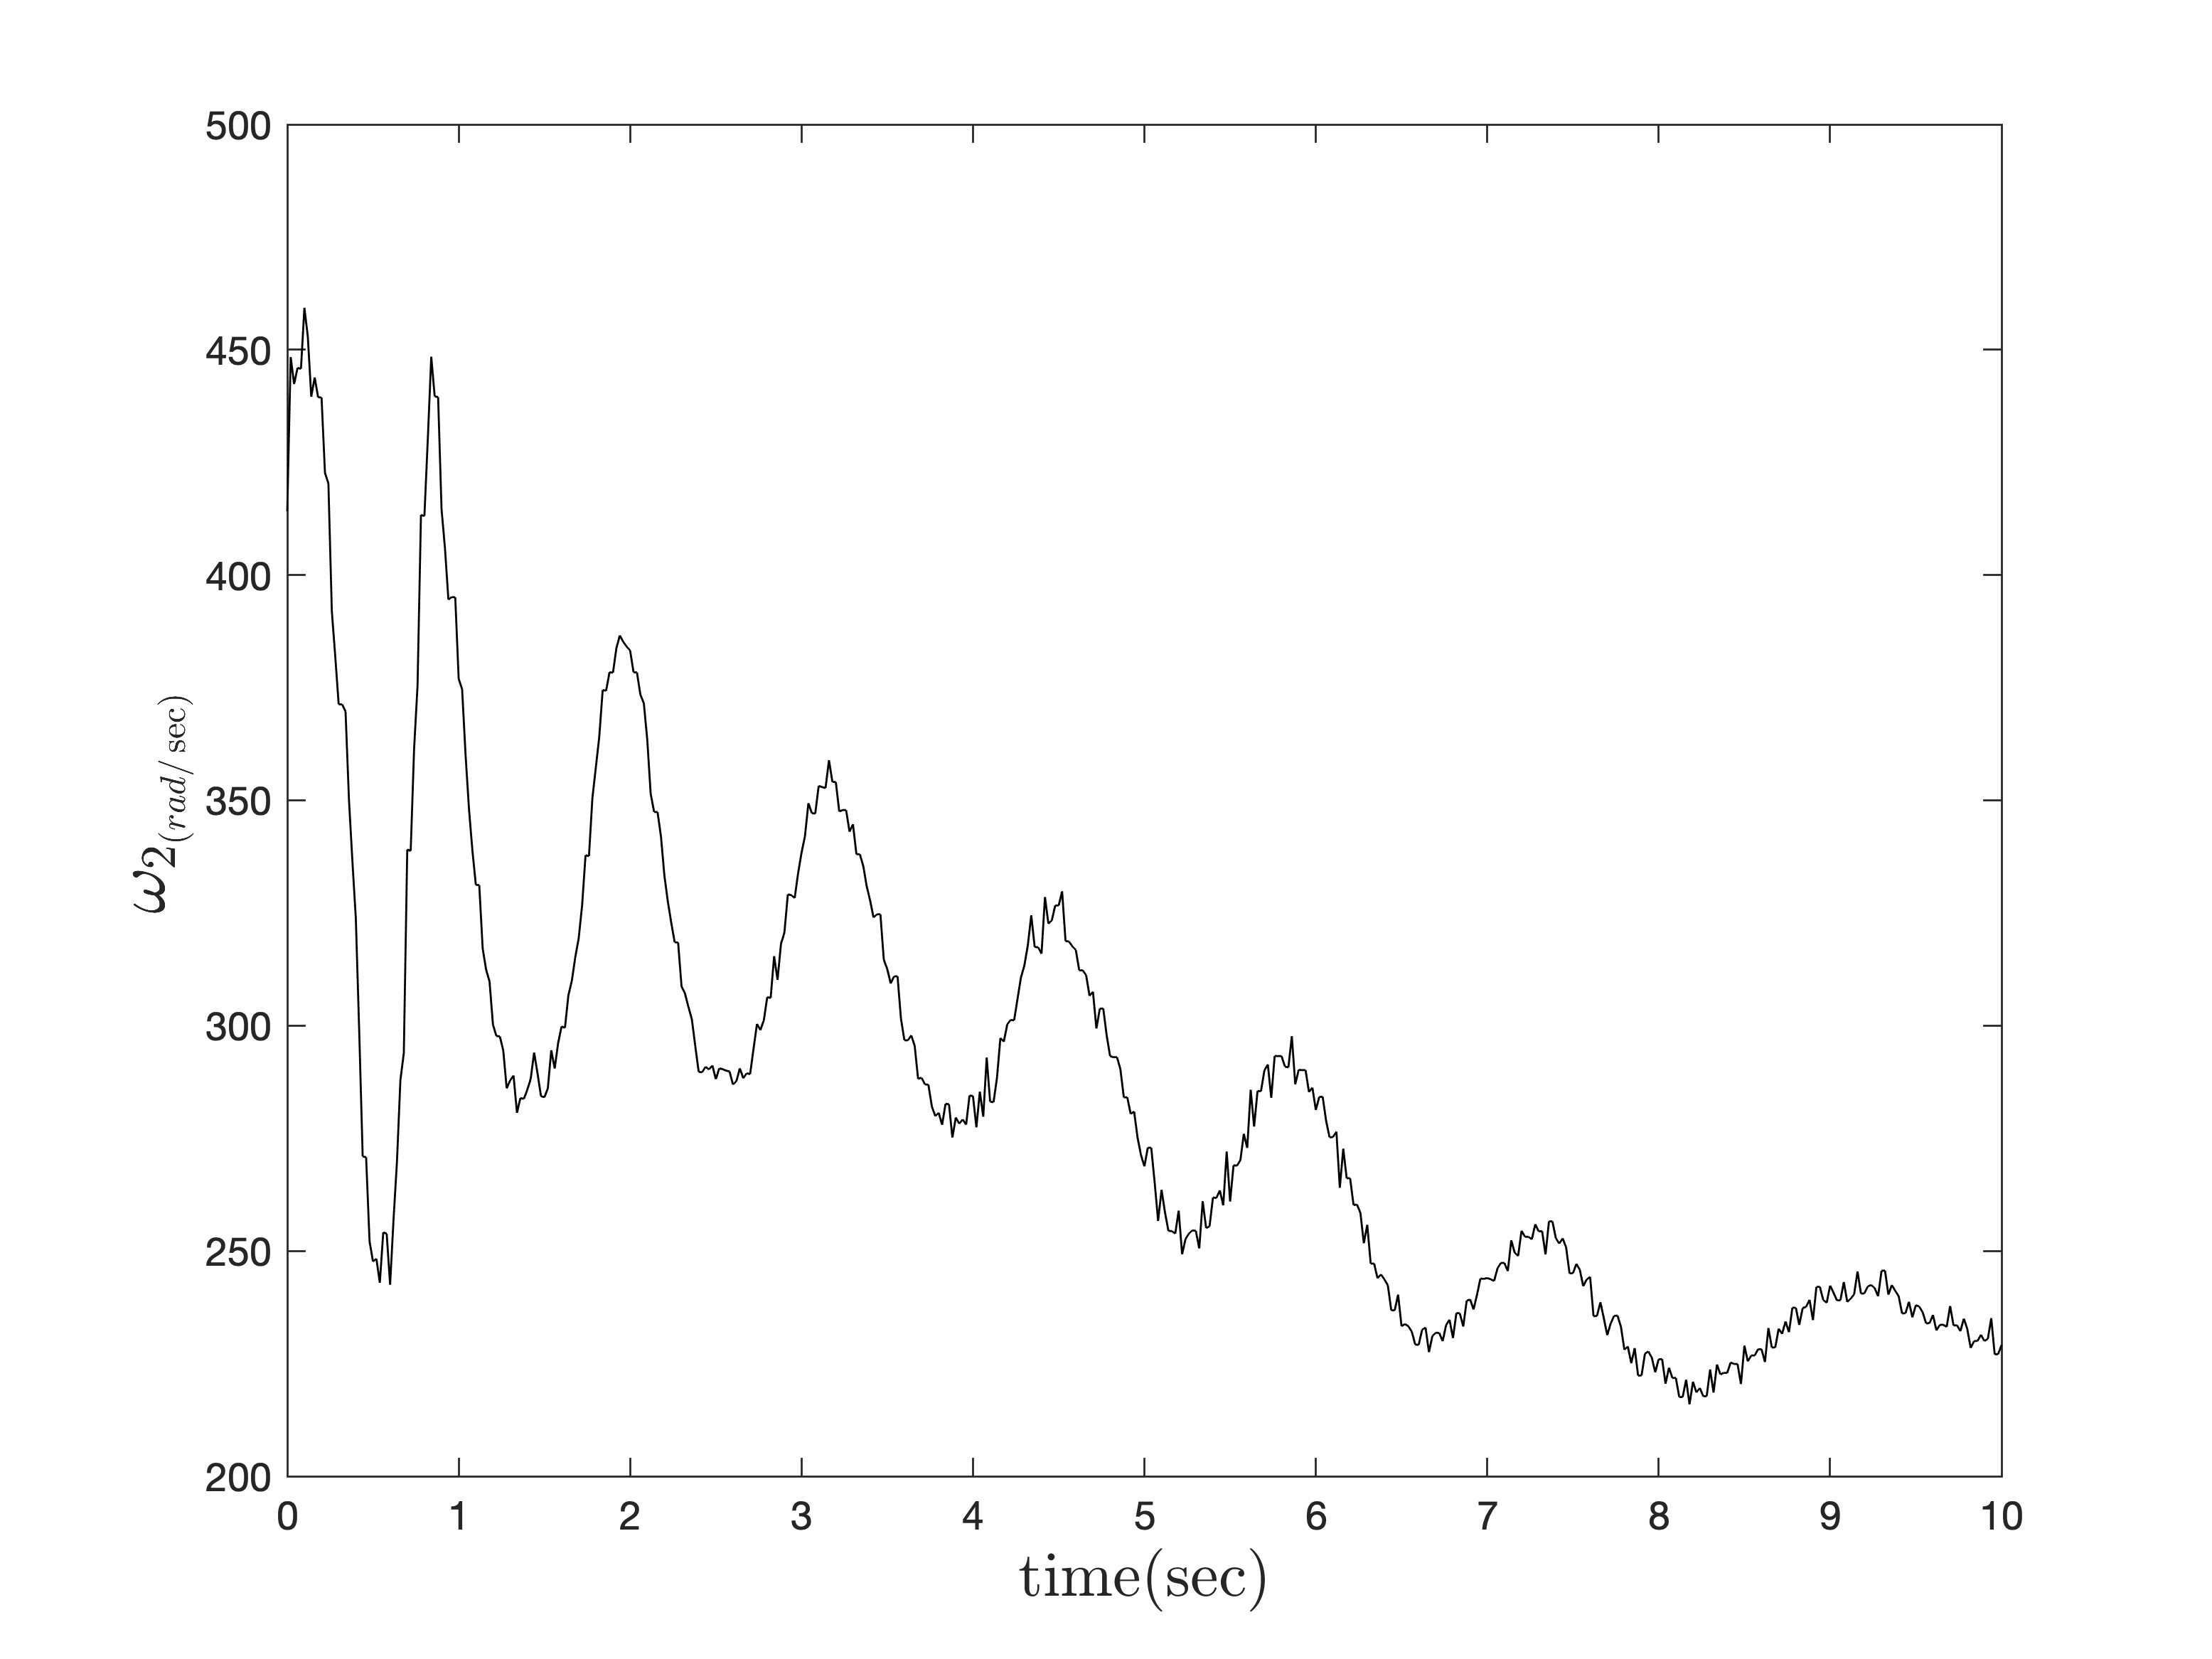
\includegraphics[width=.45\linewidth]{../Figures/Calibration/LQIDG/MIMO/lqidg_Omega_2.png}
	}
	\subfigure[موتور شماره سه]{
		\centering
		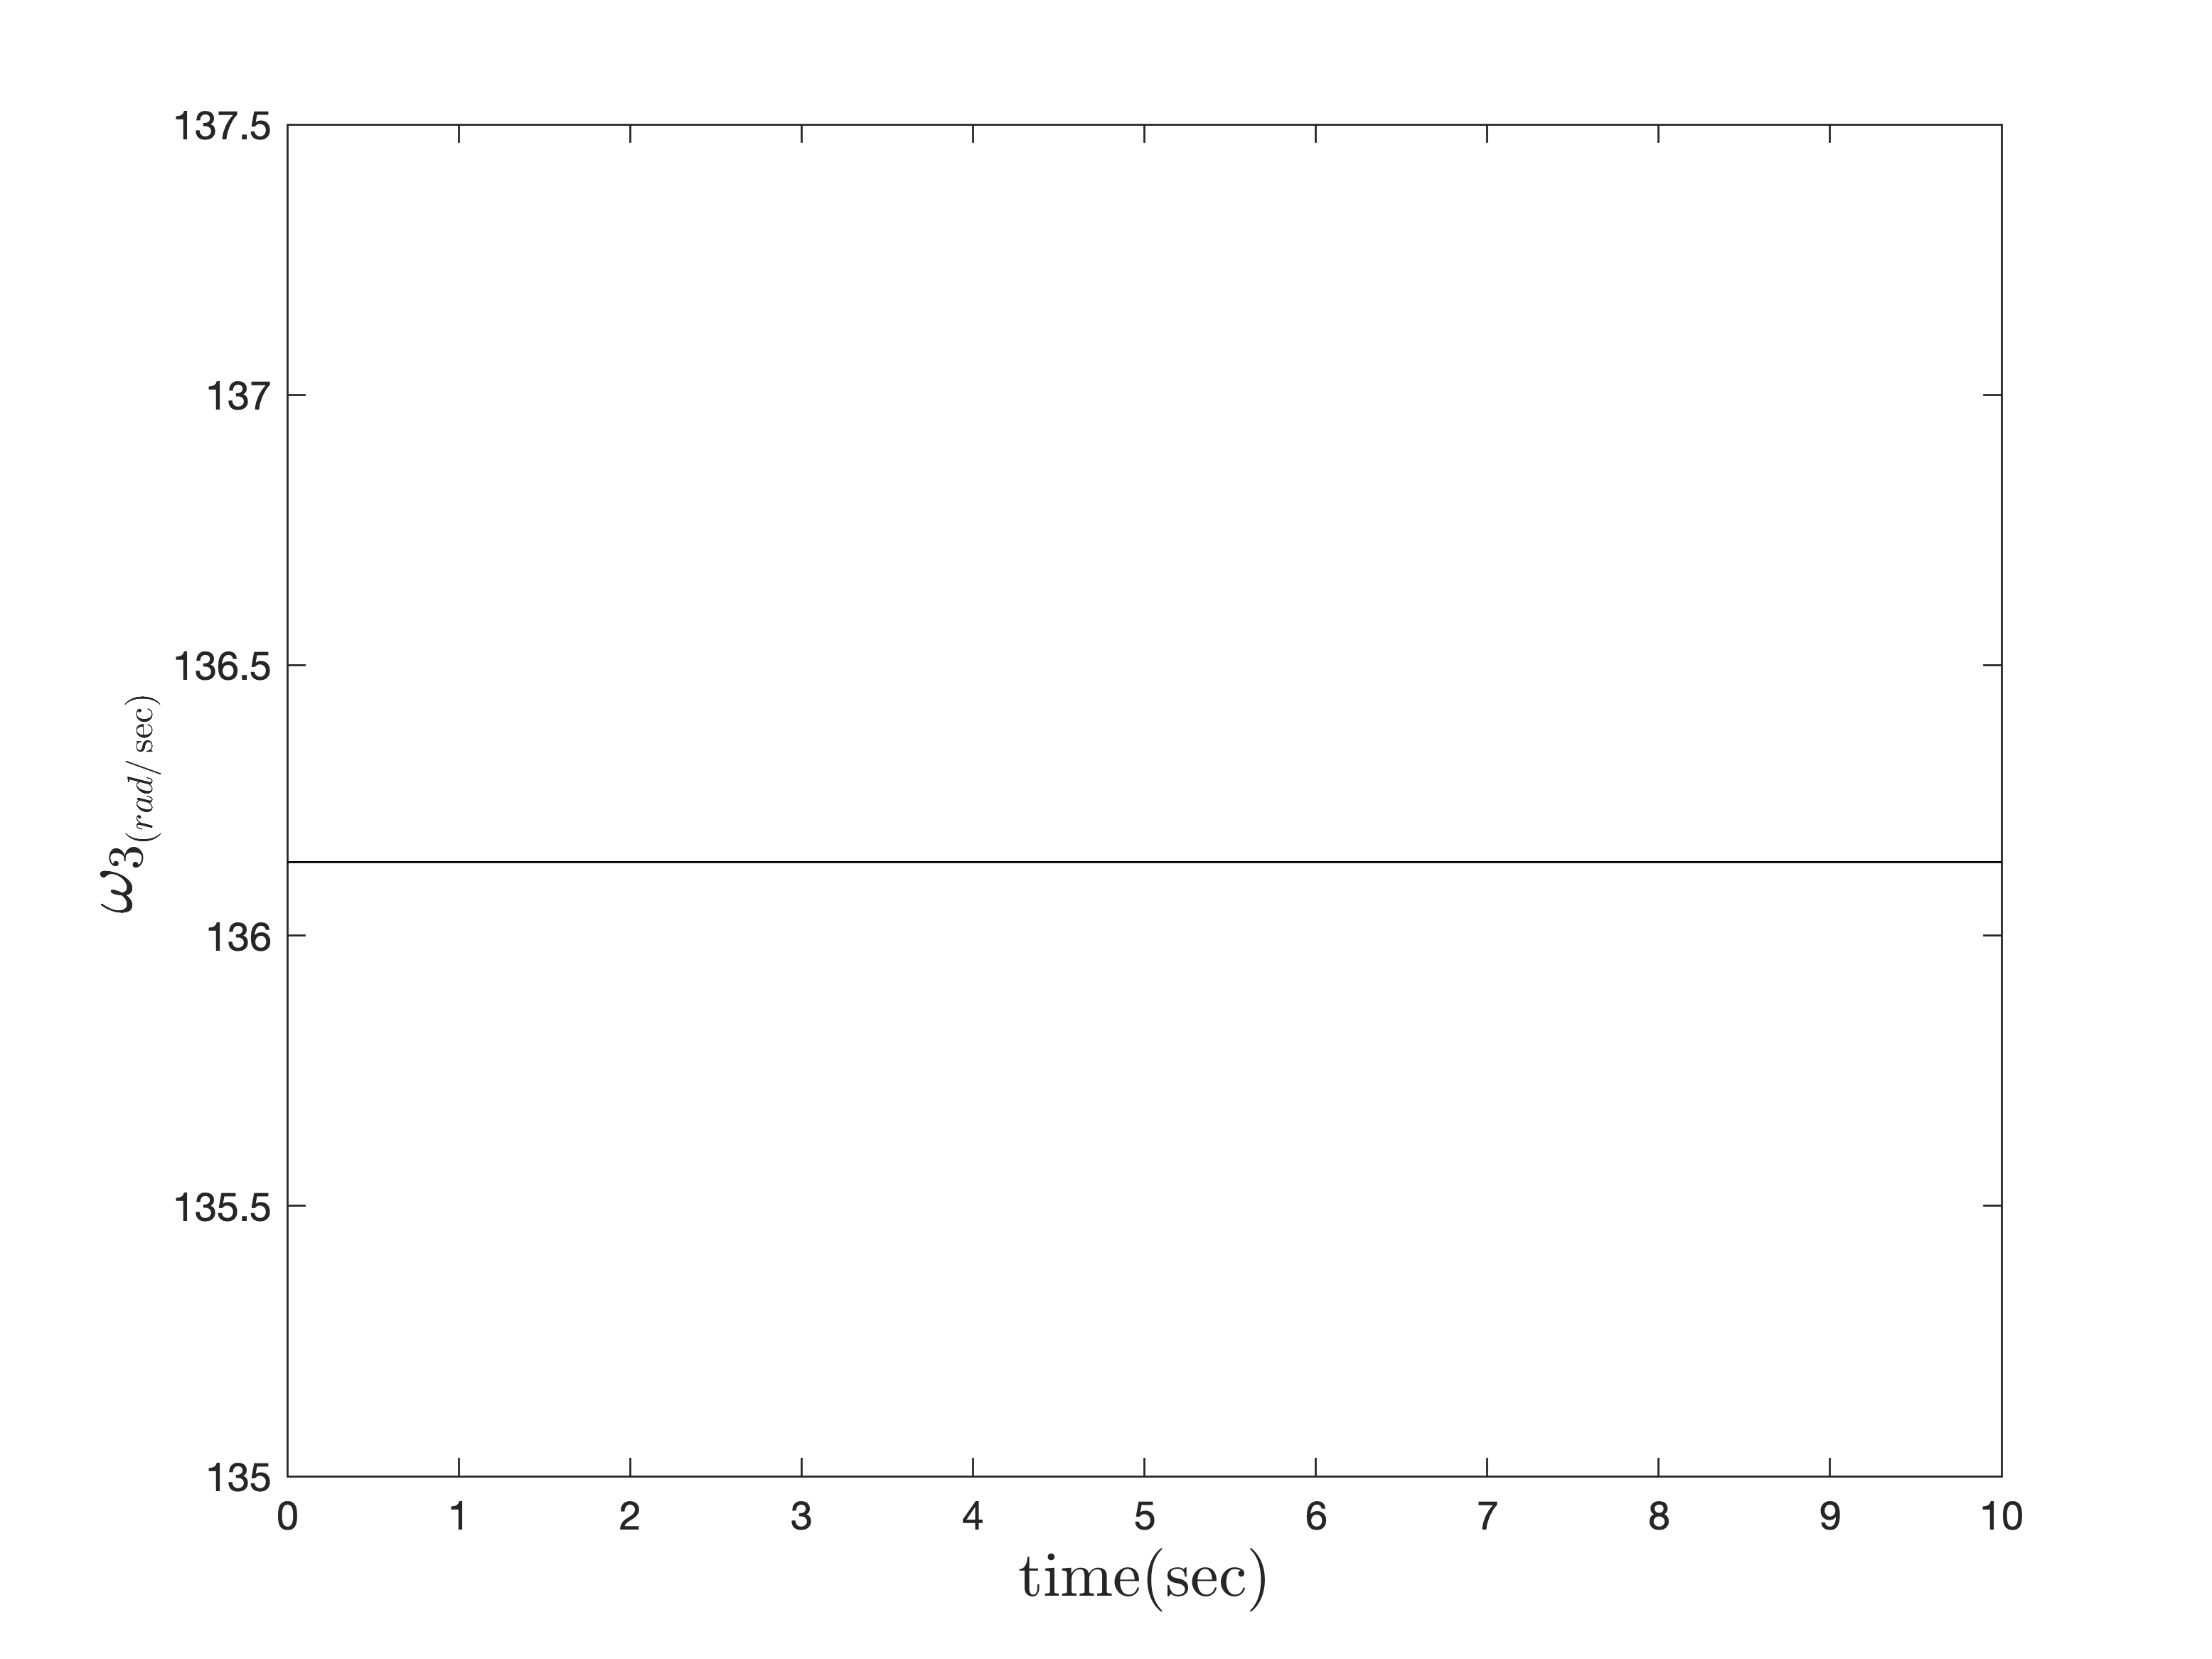
\includegraphics[width=.45\linewidth]{../Figures/Calibration/LQIDG/MIMO/lqidg_Omega_3.png}
	}
	\subfigure[موتور شماره چهار]{
		\centering
		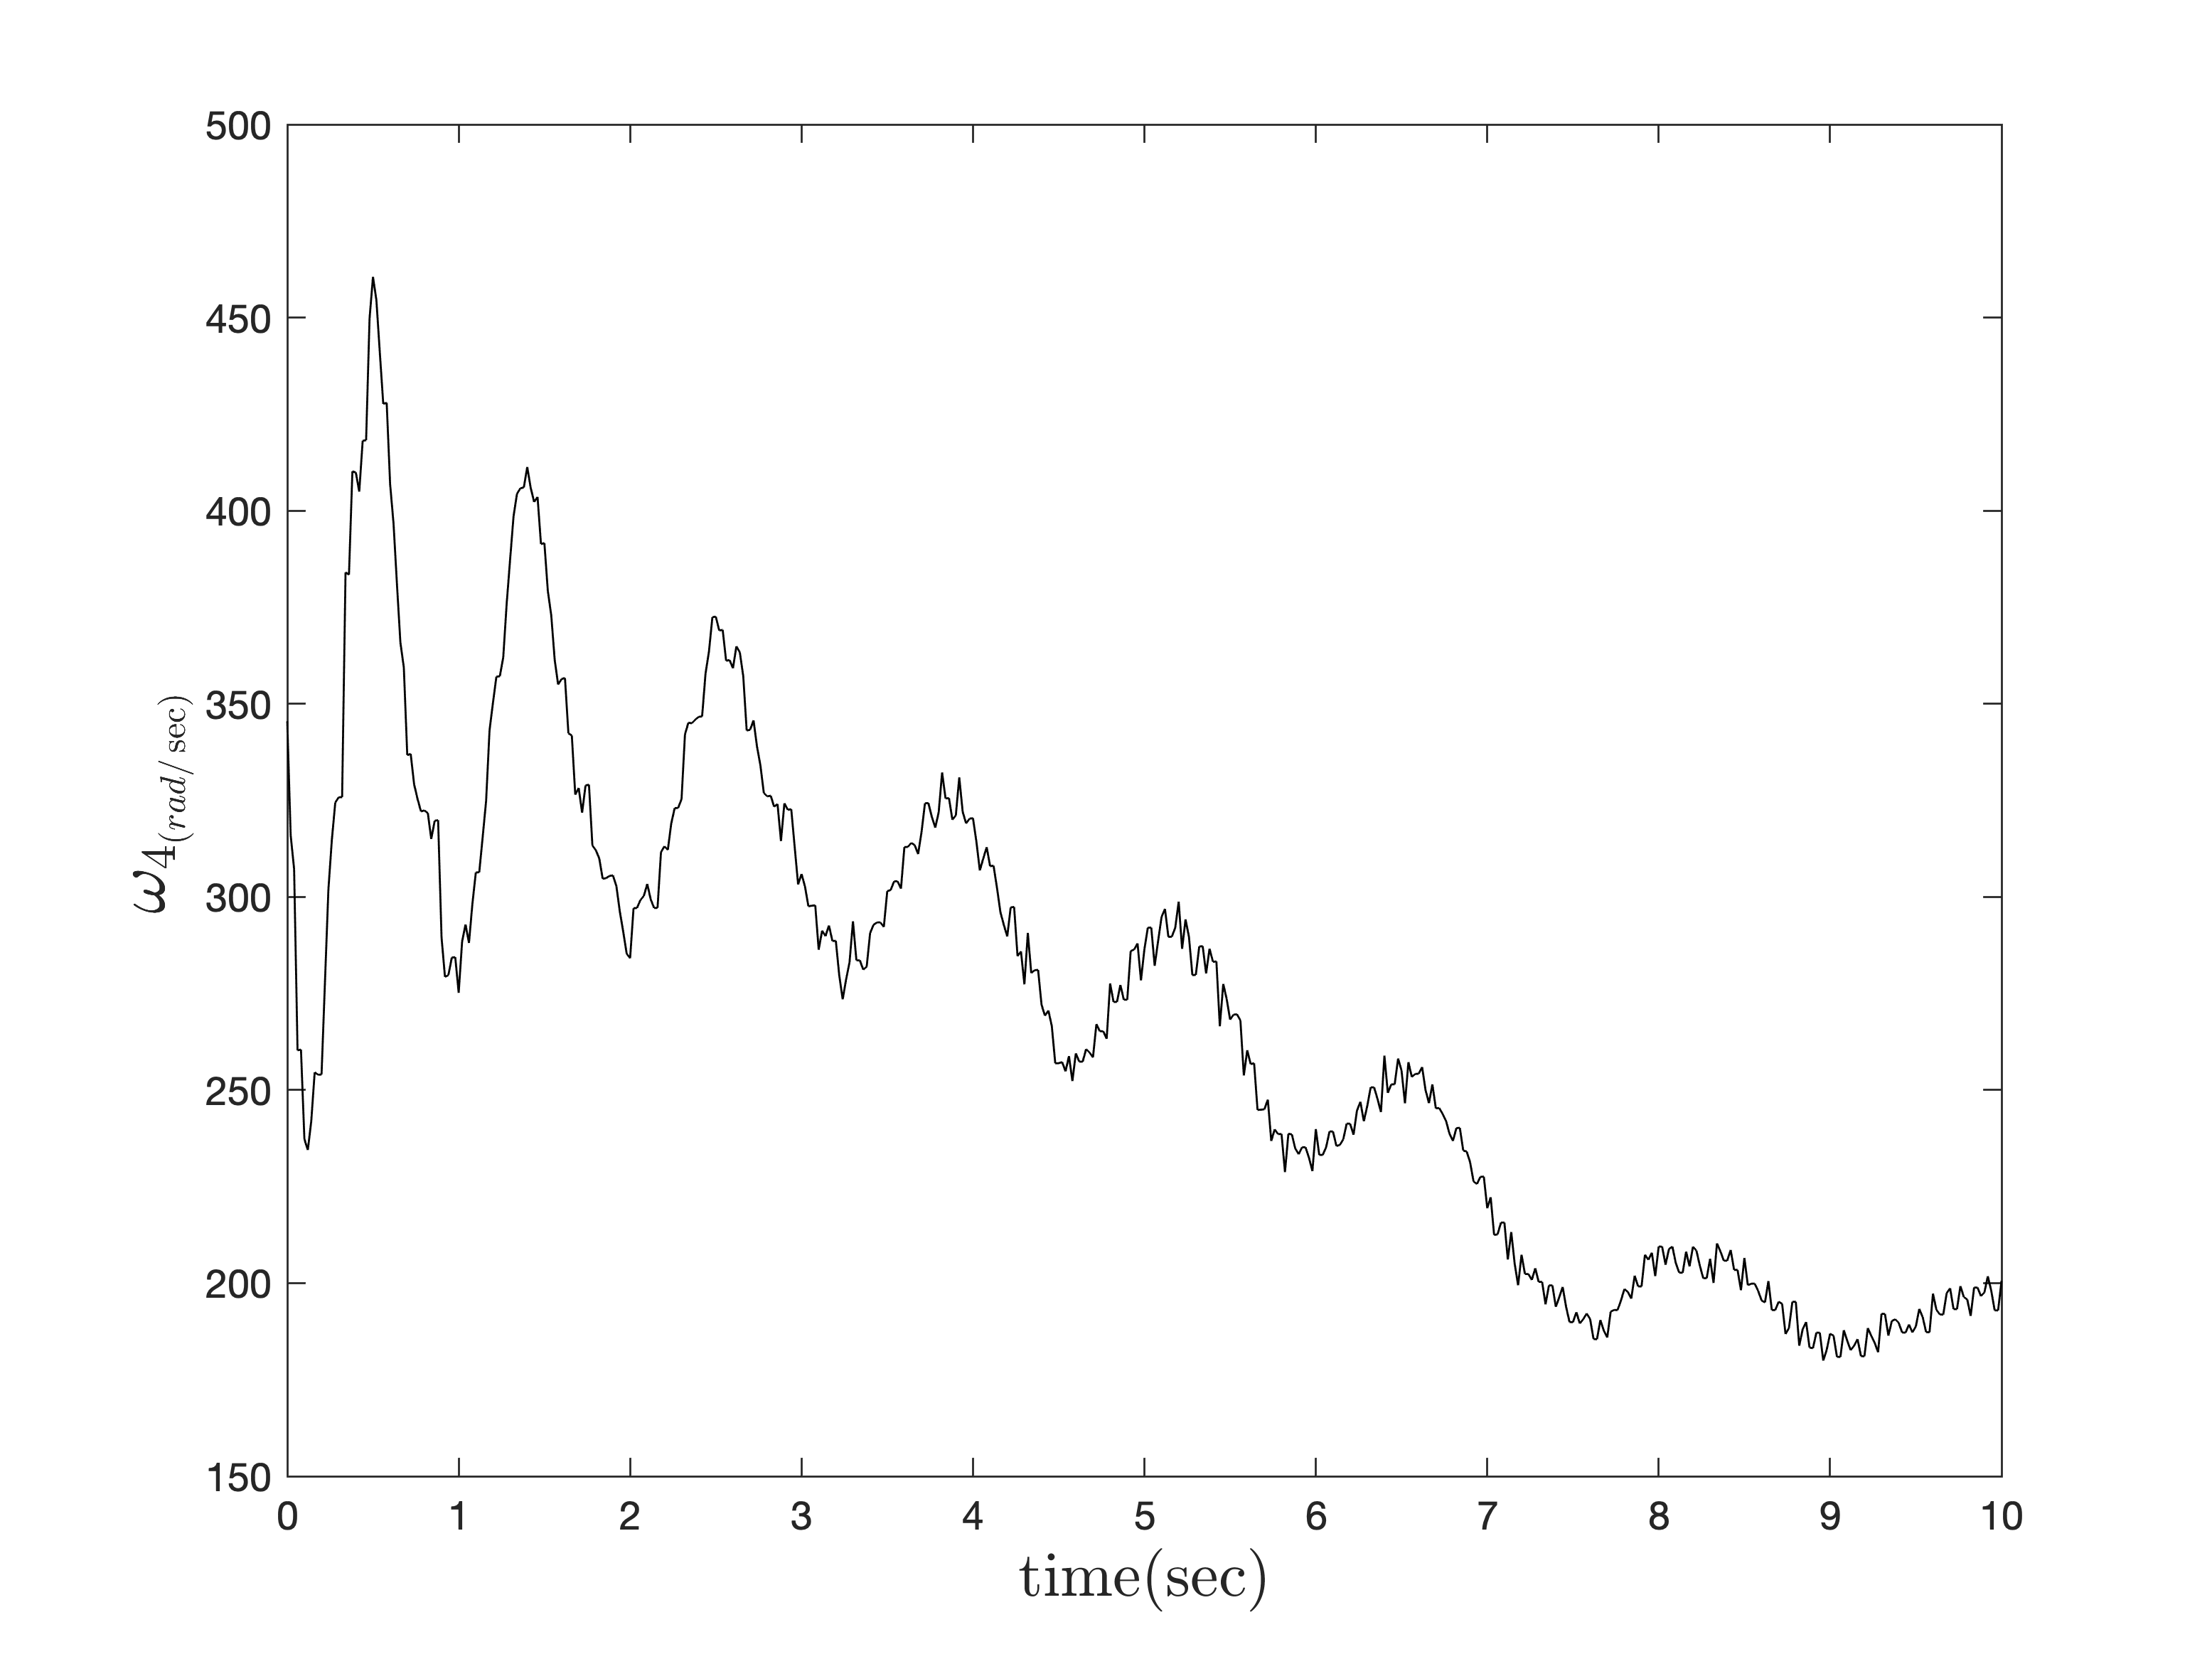
\includegraphics[width=.45\linewidth]{../Figures/Calibration/LQIDG/MIMO/lqidg_Omega_4.png}
	}
	\caption{‫‪فرمان کنترلی موتورها در کنترل وضعیت (تعقیب ورودی صفر)}
\end{figure}
